% =============================================================================
% CANONICAL VOCABULARY, DEFINITIONS, AND NOTATION SPECIFICATION
% =============================================================================
% Every section of this manuscript must adhere strictly to the following
% systems-engineering terminology and mathematical notation:
%
% 1. INTERACTING SYSTEMS & BOUNDARY PORTS
%    - Producer (Z_A) and Consumer (Z_B): Discrete component systems whose
%      interfaces are to be integrated. Avoid "sender/receiver" or "source/sink"
%      when referring to the boundary systems.
%    - Offer (O_i \in \mathcal{O}) and Need (N_j \in \mathcal{N}): Directional
%      interface declarations exposed by a Producer (Offer) or required by a
%      Consumer (Need). An Offer or Need comprises one or more typed Fields.
%    - Field (f = (c, \mathbf{k}, \mathbf{d})): The atomic unit of mediated
%      information, characterized by its Semantic Color c, Flow Kinematics
%      \mathbf{k}, and Runtime Payload Metadata \mathbf{d} (representation
%      encoding \rho and provenance \pi).
%    - Message: A structured aggregation of Fields (Record, Sequence, or Choice)
%      conveyed across a port boundary.
%
% 2. SEMANTIC COLOR & FLOW KINEMATICS
%    - Semantic Color (c = (C, L, P) \in \mathcal{C}): The three-tier UDDL
%      semantic type of a Field:
%        * Conceptual Entity (C \in \mathbb{C}): Observable phenomenon and
%          entity-association path in the Conceptual Data Model (CDM).
%        * Logical Frame (L \in \mathbb{L}): Measurement system, coordinate
%          reference frame, value domain, and unit in the Logical Data Model (LDM).
%        * Platform Realization (P \in \mathbb{P}): Numerical precision, bit
%          layout, and data type in the Platform Data Model (PDM).
%    - Flow Kinematics (\mathbf{k} = (x, v, a)): The interaction flow profile
%      of a Field at a port, recording topological locus x, flow velocity v
%      (kinetic push flow v > 0 vs. stationary pull potential v = 0), and flow
%      acceleration a = \Delta v / \Delta t (impulsive mode transitions across
%      stores/pumps and rate-mismatch exposure across multi-rate boundaries).
%    - Route Carrier: The transport medium of a connection (e.g., in-process,
%      shared-memory tree, or inter-process channel), distinct from Semantic Color.
%
% 3. MEDIATION ARCHITECTURE & WYMORIAN COUPLING
%    - Technology Catalog (TYR_{\mathcal{C}}): The color-refined Wymorian
%      buildability catalog containing Producer/Consumer capabilities and
%      reusable Mediation Operators.
%    - Mediation Operator (v \in \mathcal{V}_{\text{op}}): A discrete component
%      system from TYR_{\mathcal{C}} placed on the interior of the board,
%      classified into four move families:
%        (i)   Semantic & Representation Recoloring (\Delta C, \Delta L, \Delta P, \Delta \rho)
%        (ii)  Structural Aggregation (Assemble, Disassemble, Project, Inject)
%        (iii) Computational Derivation & Filtering (Derive, Filter/Validate)
%        (iv)  Topology, Storage & Flow Mediation (Fan/Join, Store, Mode Bridge, Stale Gate)
%    - Mediation Board (\mathcal{B} = (\mathcal{O}, \mathcal{N}, \mathcal{V}_{\text{op}}, \mathcal{E}_{\text{route}})):
%      The directed mediation graph under construction.
%    - Play (\mathcal{P}): A candidate wiring on the Mediation Board, forming a
%      semantics-refined System Coupling Recipe SCR = (VSCR, CSCR).
%    - Coupled Resultant (Z_b = \mathrm{RSY}(\mathcal{P})): The unique discrete
%      system induced by synchronous composition of the Play.
%
% 4. BEHAVIORAL CONTRACTS, WINNING CONDITIONS, AND TRADE-OFF COST
%    - Input/Output Requirement (IOR = (OLR, IR, ITR, OR, OTR, ER)): Wymore's
%      problem-space behavioral specification over operational horizon TSR.
%    - Universal Live Sequence Chart (uLSC, \mathcal{L}(IOR) = (\tau, \mathcal{P}_{\text{in}}, \mathcal{A}_{\text{out}})):
%      Behavioral contract pairing a cold Pre-Chart trigger
%      (\mathcal{P}_{\text{in}}) with a hot Main-Chart guarantee (\mathcal{A}_{\text{out}}).
%    - Hot Breach: Any violation of the Main-Chart value envelope, delivery
%      deadline, or quiet-tick silence obligation following Pre-Chart activation.
%    - Three-Tier Winning Condition:
%        * Tier 1 (Static Semantic & Structural Compatibility): Complete Field
%          coverage with aligned Semantic Colors (C, L, P), representations \rho,
%          and provenance \pi.
%        * Tier 2 (Flow & Kinematic Compatibility): Mutually compatible push/pull
%          transfer modes, positive buffer capacities, and consistent time bases.
%        * Tier 3 (Behavioral Contract Satisfaction): Zero Hot Breaches of
%          \mathcal{L}(IOR) by the Coupled Resultant Z_b over the verification
%          suite ITR_{\text{test}} (and across all trajectories in the certified
%          symbolic fragment).
%    - Integration Cost Functional (\mathcal{J}(\mathcal{P})) and Fitness Score (\mathcal{S}(\mathcal{P})):
%      Generalized Wymorian trade-off functional combining Tier 1/2 frontier
%      potentials, Static Construction Cost C_{\text{static}}, Dynamic Operational
%      Cost C_{\text{dyn}}, and Behavioral Breach Penalty C_{\text{breach}},
%      governed by axioms (A1)--(A7).
%    - uLSC Reward Machine (\mathcal{M}_{\text{LSC}}): The finite-state monitor
%      automaton compiled from \mathcal{L}(IOR) whose state u_t augments the
%      environment state \tilde{s}_t = (s_t, u_t) to restore the Markov property.
% =============================================================================

\documentclass{cser27}

% Additional packages for formal definitions, tables, and TikZ diagrams
\usepackage{amsthm}
\usepackage{tabularx}
\usepackage{enumitem}
\usepackage{xcolor}
\usepackage{tikz}
\usetikzlibrary{positioning,arrows.meta,fit,calc,shapes.geometric,backgrounds,decorations.pathreplacing}

% Paragraph formatting: remove indentation and add inter-paragraph spacing
\setlength{\parindent}{0pt}
\setlength{\parskip}{6pt plus 2pt minus 1pt}

% Shared color palette for diagrams
\definecolor{techNavy}{HTML}{1F4E79}
\definecolor{compBorder}{HTML}{343A40}
\definecolor{compFill}{HTML}{F8F9FA}
\definecolor{wireInk}{HTML}{212529}
\definecolor{boundGreen}{HTML}{2B8A3E}
\definecolor{fsrBlue}{HTML}{1864AB}
\definecolor{bsrTeal}{HTML}{087F5B}
\definecolor{poiPurple}{HTML}{5F3DC4}
\definecolor{shelfSlate}{HTML}{495057}
\definecolor{accentAmber}{HTML}{D97706}
\definecolor{hotRed}{HTML}{C92A2A}
\definecolor{coldBlue}{HTML}{1864AB}

% Theorem-like environments
\newtheorem{theorem}{Theorem}
\newtheorem{proposition}{Proposition}
\theoremstyle{definition}
\newtheorem{definition}{Definition}

% Bibliography file
\addbibresource{refs.bib}

% Paper Title
\title{The Integration Game: Automatic System Integration Inspired by T3SD}

% Authors & Affiliations
\author[a]{Nicholas McKibben}
\author[b]{Michael Mendoza}
\author[c]{Chris Allport}
\author[d]{Larry Head}
\author[e]{Alejandro Salado}

\affil[a]{Department of Systems \& Industrial Engineering, University of Arizona; \href{mailto:mckib2@arizona.edu}{mckib2@arizona.edu}; Skayl; \href{mailto:nicholas@skayl.com}{nicholas@skayl.com}}
\affil[b]{Skayl; \href{mailto:michael@skayl.com}{michael@skayl.com}}
\affil[c]{Skayl; \href{mailto:chris@skayl.com}{chris@skayl.com}}
\affil[d]{Department of Systems \& Industrial Engineering, University of Arizona; \href{mailto:klhead@arizona.edu}{klhead@arizona.edu}}
\affil[e]{Department of Systems \& Industrial Engineering, University of Arizona; \href{mailto:alejandrosalado@arizona.edu}{alejandrosalado@arizona.edu}}

\begin{document}

\maketitle

\begin{abstract}
The adoption of a Modular Open Systems Approach (MOSA) is intended to enable rapid capability insertion and multi-vendor interoperability across complex cyber-physical systems.  In practice, however, conformance to open architectural standards alone has not yielded plug-and-play integration: modular interfaces routinely diverge across semantics, measurement frames, platform encodings, and interaction dynamics.  Resolving these discrepancies remains a predominantly manual and often costly systems engineering activity.  To this end, we introduce \emph{The Integration Game}, a methodology for automated, semantically-enabled system integration based on A.~Wayne Wymore's Tricotyledon Theory of System Design (T3SD) using ontologies modeled using the Open Universal Domain Description Language (UDDL)\textsuperscript{\textregistered}.  We formulate data Producers, Consumers, and Mediation Operators as Wymorian buildable technologies in which interfaces are typed by a multi-dimensional Semantic Color (Conceptual, Logical, and Platform) together with Flow Kinematics.  Behavioral satisfiability of the Coupled Resultant is evaluated against an Input/Output Requirement (IOR), represented by a Universal Live Sequence Chart (uLSC).  We use a finite-state Reward Machine and trajectory evaluation with Counterexample-Guided Inductive Synthesis (CEGIS) to guide automated system integration, demonstrating across a fifteen-scenario verification suite that learning-guided synthesis reliably finds satisfiable and efficient system couplings under MOSA principles.
\end{abstract}

\keywords{modular open systems approach, systems integration, Tricotyledon Theory of System Design, UDDL, Live Sequence Charts, reinforcement learning}

% Modular Sections
\section{Introduction} \label{sec:intro}

Modern systems engineering is increasingly shaped by the mandate to adopt a Modular Open Systems Approach (MOSA) in the acquisition, architecture, and sustainment of complex cyber-physical systems~\cite{esper2019modular, zimmerman2019considerations}. Long-range digital-engineering visions similarly emphasize composable, model-based practice across the system lifecycle~\cite{INCOSE2035}. Reference architectures such as the Future Airborne Capability Environment (FACE)\textsuperscript{\textregistered} Technical Standard~\cite{OpenGroup2023FACE}, the Sensor Open Systems Architecture (SOSA)\textsuperscript{\textregistered} Reference Architecture~\cite{SOSAConsortium2023}, and Open Mission Systems / Universal Command and Control Interface (OMS/UCI)~\cite{esper2019modular, tokar2017osa} seek to replace monolithic, vendor-locked baselines with modular ecosystems in which hardware and software capabilities can be independently developed, inserted, and upgraded. Yet operational experience across aerospace, defense, and autonomous systems demonstrates that standardized transport buses and open interface boundaries do not, by themselves, deliver rapid or automated systems integration~\cite{madni2014system}. Even when two subsystems conform to the same reference standard, integrating an upstream \emph{Producer} capability with a downstream \emph{Consumer} capability routinely demands substantial manual engineering effort to reconcile discrepancies in domain meaning, coordinate reference frames, units of measure, wire-level type encodings, and asynchronous interaction timing.

At its core, this integration bottleneck reflects a structural division in how current model-based systems engineering (MBSE) methodologies represent interfaces. Existing formalisms largely separate \emph{static data semantics} from \emph{dynamic system behavior} and \emph{architectural trade-offs}. On the semantic side, standards such as the Open Universal Domain Description Language (UDDL)\textsuperscript{\textregistered}~\cite{OpenGroup2023UDDL} separate domain meaning from measurement convention and machine representation across conceptual, logical, and platform layers, enabling ontology alignment and query-translation algorithms to identify static correspondences between heterogeneous data models~\cite{mckibben2026alignment, mckibben2026nearring}. Identifying that two interface elements refer to related domain concepts, however, does not synthesize the stateful mediation architecture needed to couple them dynamically—such as buffering a high-rate pushed sensor stream for an on-demand guidance consumer, correlating asynchronous attitude and position reports to rotate reference frames, or bounding numerical precision loss and staleness under real-time execution constraints. Conversely, formal systems-theoretic frameworks—most notably A.~Wayne Wymore's Tricotyledon Theory of System Design (T3SD)~\cite{Wymore1993}—provide a rigorous algebra for coupling discrete component systems from a technology catalog to satisfy trajectory-level input/output requirements, but treat component ports as unstructured set-theoretic alphabets devoid of domain semantics.

Viewed through a systems-theoretic lens, a MOSA component ecosystem naturally mirrors Wymore's buildability formulation: the set of available Producer capabilities, Consumer capabilities, and reusable Mediation Operators constitutes a \emph{Technology Catalog}, and a concrete integration architecture is a \emph{System Coupling Recipe} whose synchronous composition yields a closed-loop \emph{Coupled Resultant}. In classical T3SD, certifying that a coupled assembly satisfies a behavioral specification requires manually designing the coupling recipe and constructing a surjective system homomorphism onto an abstract functional model—a manual effort that does not scale to combinatorial integration spaces or evolving component catalogs. If the port compatibility constraints of the Technology Catalog are enriched with multi-tier UDDL Semantic Colors and Flow Kinematics, however, the synthesis of a valid mediation architecture—and the online regulation of its runtime traffic—can be cast as a well-defined sequential decision problem over a formal design space.

This paper investigates whether framing semantically enabled MOSA integration as a formal game over a semantics-refined Wymorian buildability space provides a rigorous foundation for automated verification and learning-guided synthesis. Specifically, we organize our inquiry around three research questions:
\begin{enumerate}[label=\textbf{RQ\arabic*:}, leftmargin=2.8em, topsep=3pt, itemsep=2pt]
    \item \emph{Formalization of Semantic-Behavioral Integration:} How can system integration under a Modular Open Systems Approach be formalized when Producer Offers and Consumer Needs diverge simultaneously across conceptual entities, logical measurement frames, platform encodings, and interaction flow kinematics?
    \item \emph{Trajectory-Level Behavioral Satisfiability:} What formal conditions ensure that a synthesized mediation architecture not only aligns static interface types and flow mechanics, but also satisfies dynamic, trajectory-level behavioral contracts without overfitting finite test scenarios?
    \item \emph{Learning-Guided Architecture Synthesis and Control:} How can reinforcement learning leverage multi-tier semantic structure, axiomatic cost trade-offs, and assertional behavioral monitors to navigate the combinatorial space of coupling recipes offline and regulate fault-tolerant mediation policies online?
\end{enumerate}

To address these questions, we introduce \emph{The Integration Game}, a systems-theoretic methodology for dynamic interface mediation. Rather than treating interface compatibility as a static documentation checklist, we synthesize UDDL's three-tier data semantics, Wymore's T3SD coupling algebra, and Universal Live Sequence Charts (uLSCs)~\cite{DammHarel2001} into an executable design framework. Each atomic \emph{Field} exposed at a component boundary is typed by a three-axis \emph{Semantic Color} $c = (C, L, P)$ together with its \emph{Flow Kinematics} $\mathbf{k} = (x, v, a)$ and payload metadata. Legal moves on the \emph{Mediation Board} correspond to primitive \emph{Mediation Operators} that recolor Fields, aggregate or decompose Message structures, derive fused observables, buffer state, and bridge asynchronous interaction modes. To evaluate behavioral correctness without manual homomorphism proofs, we compile Wymorian Input/Output Requirements ($IOR$s) into assertional uLSCs and prove their behavioral equivalence. We then formulate a generalized \emph{Integration Cost Functional} governed by seven technology-independent axioms, and show how compiling the uLSC into a finite-state Reward Machine~\cite{ToroIcarte2022} paired with Counterexample-Guided Inductive Synthesis (CEGIS) enables Reinforcement Learning (RL) agents to synthesize verified mediation architectures offline and adapt routing policies online.

The remainder of the paper is organized as follows. Section~\ref{sec:background} establishes the theoretical foundations of UDDL data semantics, Wymore's T3SD cotyledons, and Universal Live Sequence Charts, and situates our contribution relative to prior work. Section~\ref{sec:methodology} develops the formal model of \emph{The Integration Game}, including typed Wymorian coupling, the taxonomy of Mediation Operators, the Three-Tier Winning Condition, the axiomatic Integration Cost Functional, and the Reward Machine / CEGIS learning formulation. Section~\ref{sec:results} evaluates the methodology across a fifteen-scenario progressive benchmark suite, reporting cost-sensitivity audits, symbolic fragment verification, offline synthesis generalization, and online fault-recovery performance. Section~\ref{sec:discussion} examines the systems-engineering implications, decidability boundaries, and methodological scope of the approach, and Section~\ref{sec:conclusion} concludes.

\section{Background and Theoretical Foundations} \label{sec:background}

\subsection{Data Semantics and the UDDL Three-Tier Architecture} \label{sec:bg-uddl}

Open architecture standards such as FACE and SOSA~\cite{OpenGroup2023FACE, SOSAConsortium2023} mandate shared data modeling frameworks because syntactic interface definitions alone (such as Interface Definition Language structures) cannot guarantee semantic interoperability. Two subsystems may exchange identical 32-bit floating-point vectors while disagreeing on whether those values represent geodetic coordinates or body-frame velocities, whether angles are measured in radians or degrees, or whether the reported quantity characterizes the host vehicle or a tracked target. To eliminate such ambiguities, the Open Universal Domain Description Language (UDDL)\textsuperscript{\textregistered} defines a three-tier data modeling architecture that separates domain meaning from measurement convention and machine representation~\cite{OpenGroup2023UDDL}:

\begin{itemize}[topsep=2pt, itemsep=1pt, leftmargin=1.8em]
    \item \textbf{Conceptual Data Model (CDM):} Captures abstract domain phenomena independent of measurement or computational representation. Its axiomatic primitives are \emph{Observables} (fundamental phenomena such as position, velocity, or temperature) and \emph{Basis Entities}. Domain concepts are modeled as \emph{Entities} (which compose Observables or other Entities via directed \emph{Compositions}) and \emph{Associations} (reified $n$-ary relations over ordered \emph{Participant Paths}). A conceptual \emph{Query} projects characteristics along navigational paths through the CDM to establish the exact semantic context of a datum (e.g., the position of a sensor mounted on an aircraft)~\cite{OpenGroup2023UDDL}. Multiplex-graph and near-semiring formalizations of these constructs appear in~\cite{mckibben2026multiplex, mckibben2026nearring}.
    \item \textbf{Logical Data Model (LDM):} Realizes conceptual elements by supplying the quantitative frames of reference required to interpret values, specifying \emph{Measurement Systems}, \emph{Coordinate Systems}, \emph{Reference Points}, \emph{Value Domains}, and \emph{Units} (e.g., WGS84 geodetic coordinates versus an aircraft body-centered North--East--Down frame). Multiple LDM elements may realize a single CDM element.
    \item \textbf{Platform Data Model (PDM):} Realizes logical elements in concrete computational representations, specifying primitive data types, bit layouts, endianness, and numerical precision (such as IEEE-754 32-bit versus 64-bit floating-point layouts). Multiple PDM elements may realize a single LDM element.
\end{itemize}

\begin{figure}[t]
\centering
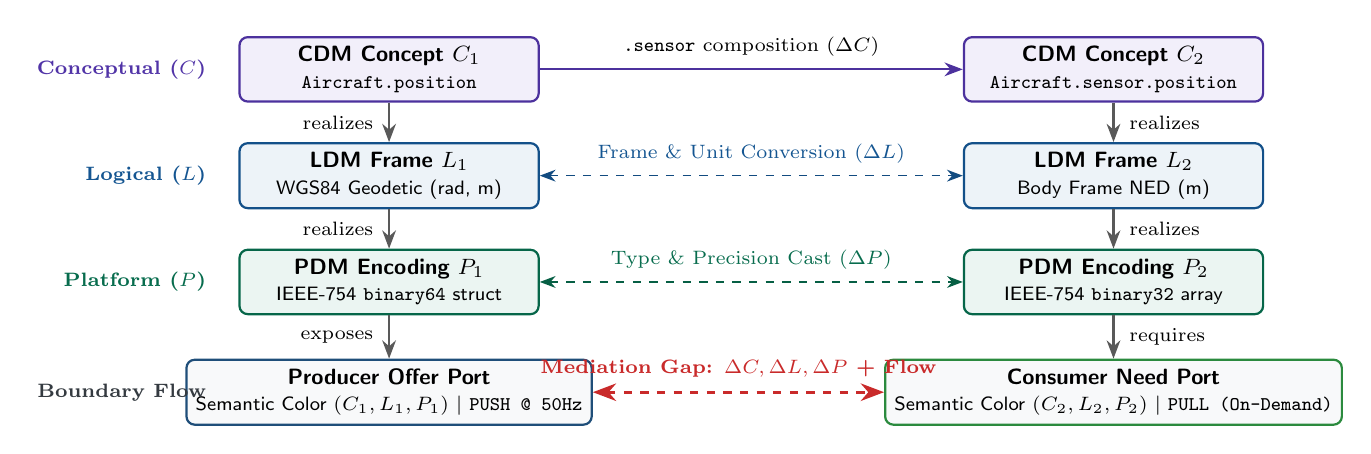
\begin{tikzpicture}[
    >=Stealth,
    font=\footnotesize\sffamily,
    cdmnode/.style={draw=poiPurple!80!black, fill=poiPurple!8, thick, rounded corners=3pt, minimum width=3.8cm, minimum height=0.78cm, align=center},
    ldmnode/.style={draw=fsrBlue!80!black, fill=fsrBlue!8, thick, rounded corners=3pt, minimum width=3.8cm, minimum height=0.78cm, align=center},
    pdmnode/.style={draw=bsrTeal!80!black, fill=bsrTeal!8, thick, rounded corners=3pt, minimum width=3.8cm, minimum height=0.78cm, align=center},
    portbox/.style={draw=compBorder, fill=compFill, thick, rounded corners=3pt, minimum width=4.0cm, minimum height=0.82cm, align=center},
    realize/.style={->, thick, draw=black!65},
    tierdelta/.style={<->, dashed, semithick, draw=black!50},
    gaparrow/.style={<->, very thick, dashed, draw=hotRed}
]
    % CDM Layer
    \node[cdmnode] (c1) at (0, 3.0) {\textbf{CDM Concept $C_1$}\\[0pt]\scriptsize \texttt{Aircraft.position}};
    \node[cdmnode] (c2) at (9.2, 3.0) {\textbf{CDM Concept $C_2$}\\[0pt]\scriptsize \texttt{Aircraft.sensor.position}};
    \draw[->, thick, draw=poiPurple!80!black] (c1.east) -- node[above=1pt, font=\scriptsize] {\texttt{.sensor} composition ($\Delta C$)} (c2.west);

    % LDM Layer
    \node[ldmnode] (l1) at (0, 1.65) {\textbf{LDM Frame $L_1$}\\[0pt]\scriptsize WGS84 Geodetic (rad, m)};
    \node[ldmnode] (l2) at (9.2, 1.65) {\textbf{LDM Frame $L_2$}\\[0pt]\scriptsize Body Frame NED (m)};
    \draw[tierdelta, draw=fsrBlue!75!black] (l1.east) -- node[above=1pt, font=\scriptsize, text=fsrBlue!85!black] {Frame \& Unit Conversion ($\Delta L$)} (l2.west);

    % PDM Layer
    \node[pdmnode] (p1) at (0, 0.30) {\textbf{PDM Encoding $P_1$}\\[0pt]\scriptsize IEEE-754 \texttt{binary64} struct};
    \node[pdmnode] (p2) at (9.2, 0.30) {\textbf{PDM Encoding $P_2$}\\[0pt]\scriptsize IEEE-754 \texttt{binary32} array};
    \draw[tierdelta, draw=bsrTeal!75!black] (p1.east) -- node[above=1pt, font=\scriptsize, text=bsrTeal!85!black] {Type \& Precision Cast ($\Delta P$)} (p2.west);

    % Producer Offer and Consumer Need
    \node[portbox, draw=techNavy] (offer) at (0, -1.10) {\textbf{Producer Offer Port}\\[0pt]\scriptsize Semantic Color $(C_1, L_1, P_1)$ $\vert$ \texttt{PUSH @ 50Hz}};
    \node[portbox, draw=boundGreen] (need) at (9.2, -1.10) {\textbf{Consumer Need Port}\\[0pt]\scriptsize Semantic Color $(C_2, L_2, P_2)$ $\vert$ \texttt{PULL (On-Demand)}};

    % Realization arrows
    \draw[realize] (c1) -- node[left=2pt, font=\scriptsize] {realizes} (l1);
    \draw[realize] (l1) -- node[left=2pt, font=\scriptsize] {realizes} (p1);
    \draw[realize] (p1) -- node[left=2pt, font=\scriptsize] {exposes} (offer);

    \draw[realize] (c2) -- node[right=2pt, font=\scriptsize] {realizes} (l2);
    \draw[realize] (l2) -- node[right=2pt, font=\scriptsize] {realizes} (p2);
    \draw[realize] (p2) -- node[right=2pt, font=\scriptsize] {requires} (need);

    % Integration gap
    \draw[gaparrow] (offer.east) -- node[above=1.5pt, font=\scriptsize\bfseries, text=hotRed] {Mediation Gap: $\Delta C, \Delta L, \Delta P$ + Flow} (need.west);

    % Layer labels on left
    \node[anchor=east, font=\scriptsize\bfseries, text=poiPurple!85!black] at (-2.2, 3.0) {Conceptual ($C$)};
    \node[anchor=east, font=\scriptsize\bfseries, text=fsrBlue!85!black] at (-2.2, 1.65) {Logical ($L$)};
    \node[anchor=east, font=\scriptsize\bfseries, text=bsrTeal!85!black] at (-2.2, 0.30) {Platform ($P$)};
    \node[anchor=east, font=\scriptsize\bfseries, text=compBorder] at (-2.2, -1.10) {Boundary Flow};
\end{tikzpicture}
\caption{The three-tier UDDL refinement hierarchy---Conceptual ($C$), Logical ($L$), and Platform ($P$)---illustrating how a Producer Offer and a Consumer Need can diverge across semantic context, coordinate frame, platform data type, and interaction flow kinematics.}
\label{fig:uddl-three-tier}
\end{figure}

As illustrated in Fig.~\ref{fig:uddl-three-tier}, every atomic \emph{Field} exposed at a component boundary is characterized along its semantic dimensions by a triple $c = (C, L, P)$, which we term its \emph{Semantic Color}. Integrating a Producer Offer with a Consumer Need requires reconciling any discrepancy across $(C, L, P)$ while simultaneously mediating the temporal and kinematic mechanics of data delivery.

\subsection{Foundations of Wymore's T3SD for Modular Integration} \label{sec:bg-t3sd}

A.~Wayne Wymore's Tricotyledon Theory of System Design (T3SD) provides a rigorous mathematical foundation for systems engineering that separates problem-space behavioral requirements from solution-space component assemblies~\cite{Wymore1993}. Contemporary MBSE interpretations connect these T3SD constructs directly to formal state machines and model-based requirements engineering~\cite{salado2019wymore, salado2019mbse}. In T3SD, a \emph{discrete system} is a deterministic Moore-type port automaton defined by a quintuple $Z = (S, I, O, \delta, \rho)$, where $S$ is a nonempty state set, $I$ and $O$ are the input and output alphabets, $\delta : S \times I \to S$ is the next-state transition function, and $\rho : S \to O$ is the state readout map. Given an initial state $s_0 \in S$ and an input trajectory $f : \mathbb{N} \to I$ over discrete ticks $t \in \mathbb{N}$, iterating $\delta$ produces a state trajectory $g(t)$ (with $g(0)=s_0$ and $g(t+1)=\delta(g(t),f(t))$) and a boundary output trajectory $y_Z(s_0, f)(t) = \rho(g(t))$. Because $\rho$ depends solely on the current state $g(t)$, every discrete system obeys Moore causality: an input arriving at tick $t$ influences the readout output no earlier than tick $t+1$.

T3SD organizes system design around three interacting spaces, or \emph{cotyledons} (Fig.~\ref{fig:t3sd-mosa-bridge}):
\begin{enumerate}[topsep=2pt, itemsep=1pt, leftmargin=1.8em]
    \item \textbf{Functionality Space $\mathrm{CTL}(IOR)$:} Problem-space behavioral requirements are stated without presupposing an internal state space via an \emph{Input/Output Requirement} 6-tuple $IOR = (OLR,\allowbreak IR,\allowbreak ITR,\allowbreak OR,\allowbreak OTR,\allowbreak ER)$, where $OLR \in \mathbb{N}^+ \cup \{\infty\}$ specifies the operational length (inducing the operational time scale $TSR = \{t \in \mathbb{N} \mid t < OLR\}$), $IR$ and $OR$ are the required boundary input and output alphabets, $ITR \subseteq IR^{TSR}$ and $OTR \subseteq OR^{TSR}$ are nonempty sets of admissible input and output trajectories, and $ER : ITR \to \mathcal{P}(OTR)$ is the \emph{eligibility relation} assigning to each admissible input scenario $f \in ITR$ a nonempty envelope of acceptable output trajectories $ER(f) \subseteq OTR$. A system $Z$ initialized at $s_0 \in S$ satisfies $IOR$ over a nonempty timescale $T \subseteq TSR$, written $\mathrm{SatisfiesIOR}(Z, IOR, s_0, T)$, if for every scenario $f \in ITR$ and every total extension $h : \mathbb{N} \to IR$ agreeing with $f$ on $TSR$, there exists an eligible trajectory $g \in ER(f)$ such that $y_Z(s_0, h)(t) = g(t)$ for all $t \in T$. All satisfying designs $D_f = (Z_f, s_0, T)$ form the functionality cotyledon $\mathrm{CTL}(IOR)$.

    \item \textbf{Buildability Space $\mathrm{CTL}(TYR)$:} Solution-space architectures are assembled from a \emph{technology} catalog $TYR$ of available discrete component systems. A \emph{System Coupling Recipe} $SCR = (VSCR, CSCR)$ selects a vector of component instances $VSCR$ from $TYR$ and specifies a one-to-one connectivity relation $CSCR$ wiring internal component output ports to compatible input ports; unwired ports remain exposed at the exterior boundary. Synchronous composition of the wired components produces a unique \emph{Coupled Resultant} discrete system $Z_b = \mathrm{RSY}(SCR)$. All buildable designs $D_b = (Z_b, SCR)$ constructible from $TYR$ form the buildability cotyledon $\mathrm{CTL}(TYR)$. In a MOSA ecosystem, the catalog of modular Producer and Consumer capabilities together with reusable Mediation Operators corresponds directly to $TYR$, while a candidate integration architecture corresponds to a coupling recipe $SCR$.

    \item \textbf{Implementability Space $\mathrm{CTL}(IOR, TYR)$:} Because a buildable Coupled Resultant $Z_b = \mathrm{RSY}(SCR)$ contains concrete buffering, framing, and mediation states absent from an abstract functional specification $Z_f \in \mathrm{CTL}(IOR)$, T3SD links the two spaces via \emph{system modes} and \emph{homomorphisms}. A system $Z_m = (S_m, I_m, O_m, \delta_m, \rho_m)$ is a system mode of $Z_b$ ($Z_m \in \mathrm{SYSMO}(Z_b)$) if it embeds into $Z_b$ within an invariant operational regime. A functional system $Z_f$ is a homomorphic image of $Z_m$ ($Z_m \twoheadrightarrow Z_f$) if there exist surjective maps $(h_S, h_I, h_O)$ that commute with transitions and readouts: $h_S(\delta_m(x, p)) = \delta_f(h_S(x), h_I(p))$ and $h_O(\rho_m(x)) = \rho_f(h_S(x))$. Whenever such a mode and homomorphism exist, $Z_b$ \emph{implements} $Z_f$, placing $(D_f, D_b)$ in $\mathrm{CTL}(IOR, TYR)$. By Wymore's Theorem~6.58~\cite{Wymore1993}, when $Z_m$ and $Z_f$ share boundary alphabets $(IR, OR)$ under identity port maps, any state homomorphism $h_S$ preserves $IOR$ satisfaction: $\mathrm{SatisfiesIOR}(Z_m, IOR, s_0, T) \iff \mathrm{SatisfiesIOR}(Z_f, IOR, h_S(s_0), T)$. Consequently, if an operational mode $Z_m$ of the Coupled Resultant directly satisfies $IOR$ at its exterior ports, $Z_m$ is itself a member of $\mathrm{CTL}(IOR)$ and implements itself via the identity homomorphism, establishing implementability without requiring manual construction of an intermediate functional state machine $Z_f$. To rank competing implementable designs, T3SD supplements $IOR$ and $TYR$ with \emph{Performance Requirements} ($PR$), \emph{Cost Requirements} ($CR$), and \emph{Trade-off Requirements} ($TR$).
\end{enumerate}

\begin{figure}[t]
\centering
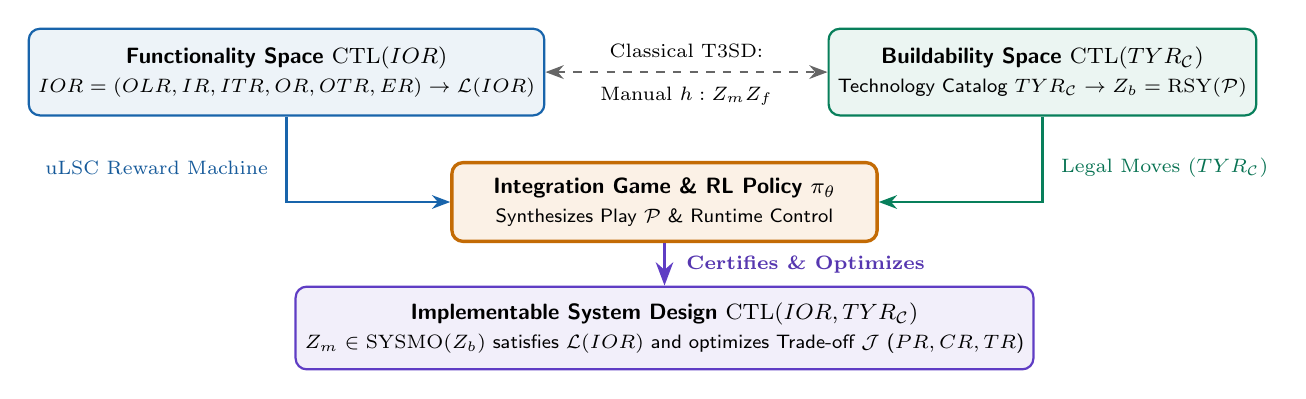
\begin{tikzpicture}[
    >=Stealth,
    font=\footnotesize\sffamily,
    fsrbox/.style={draw=fsrBlue, fill=fsrBlue!8, thick, rounded corners=4pt, minimum width=5.3cm, minimum height=1.10cm, align=center},
    bsrbox/.style={draw=bsrTeal, fill=bsrTeal!8, thick, rounded corners=4pt, minimum width=5.3cm, minimum height=1.10cm, align=center},
    isrbox/.style={draw=poiPurple, fill=poiPurple!8, thick, rounded corners=4pt, minimum width=8.6cm, minimum height=1.05cm, align=center},
    rlbox/.style={draw=accentAmber!90!black, fill=accentAmber!10, very thick, rounded corners=4pt, minimum width=5.4cm, minimum height=1.00cm, align=center}
]
    % Top Left: Functionality
    \node[fsrbox] (fsr) at (0, 2.5) {
        \textbf{Functionality Space $\mathrm{CTL}(IOR)$}\\[1pt]
        {\scriptsize $IOR = (OLR, IR, ITR, OR, OTR, ER) \to \mathcal{L}(IOR)$}
    };

    % Top Right: Buildability (MOSA)
    \node[bsrbox] (bsr) at (9.6, 2.5) {
        \textbf{Buildability Space $\mathrm{CTL}(TYR_{\mathcal{C}})$}\\[1pt]
        {\scriptsize Technology Catalog $TYR_{\mathcal{C}} \to Z_b = \mathrm{RSY}(\mathcal{P})$}
    };

    % Center: RL Engine
    \node[rlbox] (rl) at (4.8, 0.85) {
        \textbf{Integration Game \& RL Policy $\pi_\theta$}\\[1pt]
        {\scriptsize Synthesizes Play $\mathcal{P}$ \& Runtime Control}
    };

    % Bottom: Implementability
    \node[isrbox] (isr) at (4.8, -0.75) {
        \textbf{Implementable System Design $\mathrm{CTL}(IOR, TYR_{\mathcal{C}})$}\\[1pt]
        {\scriptsize $Z_m \in \mathrm{SYSMO}(Z_b)$ satisfies $\mathcal{L}(IOR)$ and optimizes Trade-off $\mathcal{J}$ ($PR, CR, TR$)}
    };

    % Arrows
    \draw[->, thick, draw=fsrBlue] (fsr.south) |- (rl.west) node[pos=0.30, left=3pt, font=\scriptsize, text=fsrBlue!90!black] {uLSC Reward Machine};
    \draw[->, thick, draw=bsrTeal] (bsr.south) |- (rl.east) node[pos=0.30, right=3pt, font=\scriptsize, text=bsrTeal!90!black] {Legal Moves ($TYR_{\mathcal{C}}$)};
    \draw[->, very thick, draw=poiPurple] (rl.south) -- node[right=4pt, font=\scriptsize\bfseries, text=poiPurple!90!black] {Certifies \& Optimizes} (isr.north);
    \draw[<->, dashed, thick, draw=black!60] (fsr.east) -- node[above=1.5pt, font=\scriptsize] {Classical T3SD:} node[below=1.5pt, font=\scriptsize] {Manual $h : Z_m \twoheadrightarrow Z_f$} (bsr.west);
\end{tikzpicture}
\caption{Adaptation of Wymore's T3SD cotyledons to automated MOSA integration. Instead of manually designing a System Coupling Recipe $SCR$ and constructing a state-space homomorphism $h$, \emph{The Integration Game} uses Reinforcement Learning guided by a uLSC Reward Machine to synthesize an implementable Play $\mathcal{P}$ and Coupled Resultant $Z_b = \mathrm{RSY}(\mathcal{P})$.}
\label{fig:t3sd-mosa-bridge}
\end{figure}

\subsection{Universal Live Sequence Charts and \texorpdfstring{$IOR$}{IOR} Correspondence} \label{sec:bg-ulsc}

While set-theoretic trajectory relations $ER \subseteq ITR \times OTR$ provide an unambiguous mathematical foundation, automated verification and learning pipelines benefit from an assertional, scenario-based representation that separates environmental trigger assumptions from mandatory system guarantees. Live Sequence Charts (LSCs)~\cite{DammHarel2001, HarelMarelly2003} extend Message Sequence Charts~\cite{ITUTZ120} with universal quantification and \emph{cold} (provisional) versus \emph{hot} (mandatory) temperatures. To encode Wymorian $IOR$s without loss of generality, we define a compact, assertional \emph{Universal LSC} fragment over two boundary lifelines—the external environment ($\mathsf{Env}$) and the system under mediation ($\mathsf{Sys}$):

\begin{definition}[Assertional Universal LSC] \label{def:ulsc}
A Universal LSC over input alphabet $IR$ and output alphabet $OR$ is a tuple $\mathcal{L} = (\tau, \mathcal{P}_{\text{in}}, \mathcal{A}_{\text{out}})$, where $\tau \subseteq \mathbb{N}$ is the discrete operational horizon, $\mathcal{P}_{\text{in}} \subseteq IR^{\mathbb{N}}$ is the \emph{cold Pre-Chart} predicate specifying the set of eligible environmental input trajectories that activate the contract, and $\mathcal{A}_{\text{out}} : IR^{\mathbb{N}} \times OR^{\mathbb{N}} \to \{\mathrm{true}, \mathrm{false}\}$ is the \emph{hot Main-Chart} relation specifying admissible input--output trajectory pairs (including value tolerances, delivery deadlines, and quiet-output \emph{silence} obligations).
\end{definition}

A discrete system $Z = (S, IR, OR, \delta, \rho)$ initialized at $s_0 \in S$ \emph{satisfies} a Universal LSC $\mathcal{L}$ on timescale $T \subseteq \tau$, written $\mathrm{SatisfiesLSC}(Z, \mathcal{L}, s_0, T)$, when $T \neq \emptyset$ and every Pre-Chart activation forces a Main-Chart fulfillment:
\begin{equation}
    \forall f \in \mathcal{P}_{\text{in}},\; \forall h \in IR^{\mathbb{N}},\; \big(\forall t \in \tau,\; h(t) = f(t)\big) \implies \exists g \in OR^{\mathbb{N}},\; \mathcal{A}_{\text{out}}(f, g) \wedge \big(\forall t \in T,\; y_Z(s_0, h)(t) = g(t)\big).
    \label{eq:lsc-sat}
\end{equation}
If an input trajectory $h$ fails to match $\mathcal{P}_{\text{in}}$ on $\tau$, the cold Pre-Chart is vacated without penalty; conversely, if the Pre-Chart matches on $\tau$ but no allowed output trajectory $g$ agrees with $y_Z(s_0, h)$ on $T$, a \emph{Hot Breach} occurs. Given any Wymorian requirement $IOR = (OLR, IR, ITR, OR, OTR, ER)$, we compile its \emph{characteristic Universal LSC} $\mathcal{L}(IOR)$ by setting $\tau = TSR(IOR)$, $\mathcal{P}_{\text{in}} = ITR$, and $\mathcal{A}_{\text{out}}(f, g) \Longleftrightarrow g \in ER(f)$ (Fig.~\ref{fig:ulsc-diagram}).

\begin{theorem}[Correspondence Between $IOR$s and Universal LSCs] \label{thm:ior-lsc}
For every Input/Output Requirement $IOR = (OLR, IR, ITR, OR, OTR, ER)$, discrete system $Z = (S, IR, OR, \delta, \rho)$, initial state $s_0 \in S$, and evaluation timescale $T \subseteq \mathbb{N}$,
\begin{equation}
    \mathrm{SatisfiesLSC}(Z, \mathcal{L}(IOR), s_0, T) \iff \mathrm{SatisfiesIOR}(Z, IOR, s_0, T).
    \label{eq:ior-lsc-equiv}
\end{equation}
Moreover, a Hot Breach occurs on an input scenario $f \in ITR$ (with extension $h$ agreeing with $f$ on $TSR$) if and only if $Z$ fails to satisfy $IOR$ on $f$.
\end{theorem}

\begin{proof}[Proof Sketch]
By definition of $\mathcal{L}(IOR)$, $\tau = TSR(IOR)$, $\mathcal{P}_{\text{in}} = ITR$, and $\mathcal{A}_{\text{out}}(f, g) \iff g \in ER(f)$. Substituting these directly into~\eqref{eq:lsc-sat} yields the exact trajectory quantification of Wymore's $\mathrm{SatisfiesIOR}$: $T \neq \emptyset$, $T \subseteq TSR(IOR)$, and for every $f \in ITR$ and extension $h$ agreeing with $f$ on $TSR(IOR)$, there exists $g \in ER(f)$ matching $y_Z(s_0, h)(t)$ at all $t \in T$. Defining $\mathcal{A}_{\text{out}}$ via full envelope membership $g \in ER(f)$ is essential: a pointwise projection requiring only $y_Z(s_0, h)(t) \in \{g(t) \mid g \in ER(f)\}$ at each tick $t$ independently is strictly weaker whenever $ER(f)$ couples outputs across ticks. Negating~\eqref{eq:lsc-sat} immediately yields the Hot Breach condition.
\end{proof}

\begin{figure}[t]
\centering
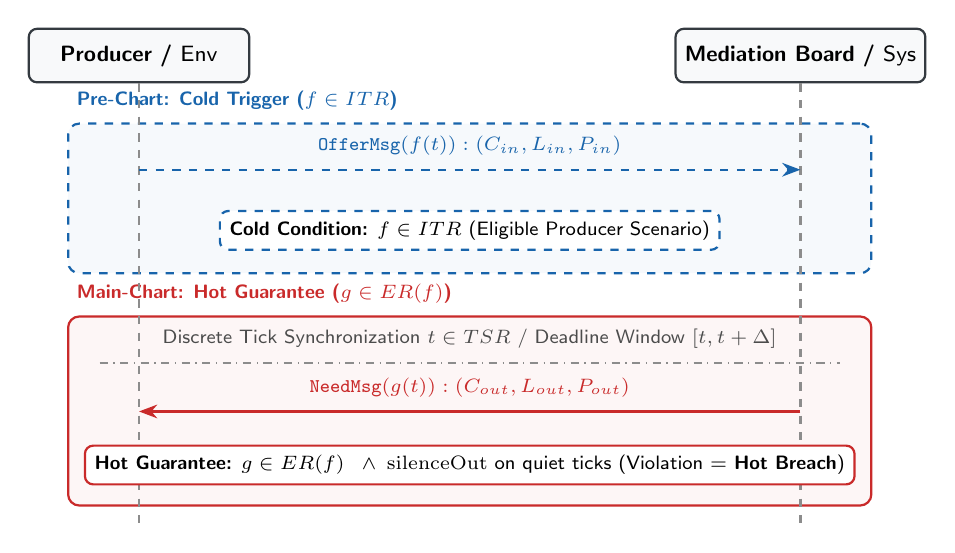
\begin{tikzpicture}[
    >=Stealth,
    font=\footnotesize\sffamily,
    lifelinehead/.style={draw=compBorder, fill=compFill, thick, rounded corners=3pt, minimum width=2.8cm, minimum height=0.68cm, align=center, font=\footnotesize\sffamily\bfseries},
    coldframe/.style={draw=coldBlue, dashed, thick, fill=coldBlue!4, rounded corners=4pt},
    hotframe/.style={draw=hotRed, solid, thick, fill=hotRed!4, rounded corners=4pt},
    lsccond/.style={draw=black!30, fill=white, rounded corners=3pt, font=\scriptsize\sffamily, inner sep=3.5pt, align=center}
]
    % Lifeline Heads
    \node[lifelinehead] (env) at (0, 0) {Producer / $\mathsf{Env}$};
    \node[lifelinehead] (sys) at (8.4, 0) {Mediation Board / $\mathsf{Sys}$};

    % Pre-Chart (Cold Trigger Region): y from -0.85 to -2.75
    \node[coldframe, minimum width=10.2cm, minimum height=1.90cm, anchor=north] (pre_box) at (4.2, -0.85) {};
    \node[font=\scriptsize\sffamily\bfseries, text=coldBlue, anchor=south west] at ([yshift=1pt]pre_box.north west)
      {Pre-Chart: Cold Trigger ($f \in ITR$)};

    % Main-Chart (Hot Guarantee Region): y from -3.30 to -5.70
    \node[hotframe, minimum width=10.2cm, minimum height=2.40cm, anchor=north] (main_box) at (4.2, -3.30) {};
    \node[font=\scriptsize\sffamily\bfseries, text=hotRed, anchor=south west] at ([yshift=1pt]main_box.north west)
      {Main-Chart: Hot Guarantee ($g \in ER(f)$)};

    % Vertical Lifeline Rays
    \draw[dashed, thick, black!45] (env.south) -- (0, -5.95);
    \draw[dashed, thick, black!45] (sys.south) -- (8.4, -5.95);

    % Cold Input Message (Env -> Sys)
    \draw[-{Stealth}, dashed, thick, draw=coldBlue] (0, -1.45) --
      node[above=1.5pt, font=\scriptsize\sffamily, text=coldBlue] {\texttt{OfferMsg}$(f(t)) : (C_{\text{in}}, L_{\text{in}}, P_{\text{in}})$} (8.4, -1.45);

    % Cold Guard Condition
    \node[lsccond, draw=coldBlue, dashed, thick] at (4.2, -2.22)
      {\textbf{Cold Condition:} $f \in ITR$ (Eligible Producer Scenario)};

    % Tick Synchronization
    \draw[dashdotted, thick, black!45] (-0.5, -3.90) --
      node[above=1.5pt, font=\scriptsize\sffamily, text=black!70] {Discrete Tick Synchronization $t \in TSR$ / Deadline Window $[t, t+\Delta]$} (8.9, -3.90);

    % Hot Output Message (Sys -> Env)
    \draw[-{Stealth}, solid, thick, draw=hotRed] (8.4, -4.52) --
      node[above=1.5pt, font=\scriptsize\sffamily, text=hotRed] {\texttt{NeedMsg}$(g(t)) : (C_{\text{out}}, L_{\text{out}}, P_{\text{out}})$} (0, -4.52);

    % Hot Envelope Condition
    \node[lsccond, draw=hotRed, solid, thick] at (4.2, -5.20)
      {\textbf{Hot Guarantee:} $g \in ER(f)$ \enspace$\wedge$\enspace $\mathrm{silenceOut}$ on quiet ticks (Violation $=$ \textbf{Hot Breach})};
\end{tikzpicture}
\caption{Diagrammatic structure of the characteristic Universal LSC $\mathcal{L}(IOR)$. A match on the dashed blue Cold Pre-Chart triggers the solid red Hot Main-Chart obligation; any violation of the output value envelope, timing window, or silence constraint induces a Hot Breach.}
\label{fig:ulsc-diagram}
\end{figure}

\subsection{Related Work} \label{sec:bg-literature}

Automating semantically enabled systems integration sits at the intersection of four research traditions that have historically developed largely in parallel (Table~\ref{tab:related-work}):

\paragraph{Schema Mapping, Ontology Alignment, and Query Translation.}
In database theory and the semantic web, integrating heterogeneous sources is classically modeled via Global-as-View (GAV), Local-as-View (LAV), and GLAV schema mappings~\cite{lenzerini2002data}, automatic schema matching~\cite{rahm2001schema}, probabilistic schema mappings~\cite{dong2009data}, and Ontology-Based Data Access (OBDA)~\cite{calvanese2007tractable, xiao2018ontology}. Within the systems engineering and MOSA literature, recent work has formalized UDDL conceptual data models as multiplex graphs~\cite{mckibben2026multiplex}, aligned disparate UDDL models via Fused Gromov--Wasserstein optimal transport~\cite{mckibben2026alignment}, and translated navigational UDDL Queries across domain models via binary integer programming over near-semirings~\cite{mckibben2026nearring}. While these methods identify static semantic correspondences between schemas, they do not synthesize stateful mediation architectures capable of transforming coordinate frames, buffering asynchronous streams, or satisfying trajectory-level temporal constraints.

\paragraph{Protocol Mediation, Interface Theories, and Formal Solvers.}
In formal methods and software architecture, component interoperability has been studied through Interface Automata~\cite{deAlfaroHenzinger2001}, assume/guarantee contracts~\cite{BenvenisteEtAl2018}, mediating connector patterns~\cite{SpalazzeseInverardi2010}, and reactive controller synthesis~\cite{PnueliRosner1989}. Satisfiability Modulo Theories (SMT) solvers such as Z3~\cite{deMouraZ32008} underpin automated verification of these interface theories, while mixed-integer linear programming has been applied to combinatorial join planning~\cite{trummer2017solving}. Purely monolithic symbolic synthesis, however, struggles to scale when integration requires combining multi-tier semantic conversions $(C, L, P)$, continuous value transformations, bounded queueing dynamics, and multi-objective cost trade-offs.

\paragraph{Reinforcement Learning and Reward Machines.}
Reinforcement learning~\cite{SuttonBarto2018} has demonstrated strong capability in navigating large discrete architectural spaces, including circuit macro placement~\cite{Mirhoseini2021} and combinatorial game search~\cite{Silver2018AlphaZero}, as well as continuous operational control via policy-gradient and actor--critic methods~\cite{Schulman2017PPO, Haarnoja2018SAC}. To bridge formal temporal specifications and RL, Toro Icarte et al.~\cite{ToroIcarte2018, ToroIcarte2022} introduced \emph{Reward Machines}: finite-state automata that expose the structure of non-Markovian tasks to the learning agent, enabling potential-based reward shaping~\cite{NgHaradaRussell1999}. Subsequent work compiles Linear Temporal Logic and related formal languages into Reward Machines for specification-guided learning~\cite{Camacho2019LTL, Pnueli1977, BaierKatoen2008}. These techniques have not previously been unified with Wymorian Input/Output Requirements, UDDL three-tier interface semantics, or MOSA system coupling.

\begin{table}[t]
\centering
\caption{Comparison of adjacent research traditions and the gap addressed by \emph{The Integration Game}.}
\label{tab:related-work}
\footnotesize
\begin{tabularx}{\linewidth}{@{}>{\raggedright\arraybackslash}p{3.1cm} >{\raggedright\arraybackslash}p{4.3cm} >{\raggedright\arraybackslash}X@{}}
\toprule
\textbf{Research Tradition} & \textbf{Primary Capabilities} & \textbf{Limitations for Dynamic MOSA Integration} \\
\midrule
Ontology Alignment \& Query Translation~\cite{rahm2001schema, lenzerini2002data, xiao2018ontology, mckibben2026alignment, mckibben2026nearring} & Aligns static conceptual schemas ($C$) and rewrites navigational queries across models. & Does not synthesize stateful flow mediation, logical/platform value transforms ($L, P$), or runtime timing guarantees. \\
\addlinespace[2pt]
Interface Automata \& Symbolic Synthesis~\cite{deAlfaroHenzinger2001, BenvenisteEtAl2018, SpalazzeseInverardi2010, deMouraZ32008} & Verifies protocol handshakes and synthesizes mediating connectors; SMT solvers support formal analysis. & Poorly suited to multi-objective cost trade-offs, multi-tier semantic distance metrics, and adaptive runtime control. \\
\addlinespace[2pt]
Classical Wymore T3SD~\cite{Wymore1993, salado2019wymore, ZeiglerPraehoferKim2000, wach2021devs} & Rigorous coupling algebra ($\mathrm{RSY}$), behavioral $IOR$s, and $PR/CR/TR$ trade-offs; DEVS provides a related discrete-event lineage. & Unstructured port alphabets (no $(C,L,P)$ semantics); relies on manual coupling design and homomorphism construction without automated search. \\
\addlinespace[2pt]
RL \& Reward Machines~\cite{Mirhoseini2021, ToroIcarte2022, Camacho2019LTL, Schulman2017PPO} & Scalable search over combinatorial graphs and non-Markovian temporal tasks. & Lacks domain-specific port typing, UDDL semantic distance metrics, and systems-theoretic buildability semantics. \\
\bottomrule
\end{tabularx}
\end{table}

\section{Methodology} \label{sec:methodology}

To make automated MOSA integration amenable to formal verification and reinforcement learning while maintaining a systems-theoretic approach, we formulate interface mediation as an \emph{Integration Game}.  The framework defines a structured design space of positions (\emph{Mediation Boards}), legal moves (\emph{Mediation Operators}), winning conditions (typing, kinematic, and behavioral satisfiability), and quantitative trade-off objectives (\emph{Integration Cost Functionals}).  Every interface element is typed by a single Stateful \emph{Color}, characterized by the UDDL data semantic layers of Section~\ref{sec:bg-uddl} along with runtime representation, flow kinematics, and provenance; behavioral obligations are expressed as uLSC contracts equivalent to Wymorian $IOR$s; and search is guided by a Reward Machine compiled from those contracts.

\subsection{Elemental Decomposition} \label{sec:meth-isomorphism}

We decompose an integration problem as follows:

\begin{enumerate}[topsep=2pt, itemsep=1pt, leftmargin=1.8em]
    \item \textbf{Producers and Consumers.} Abstractions of discrete component systems whose interfaces are to be integrated.  Producer and Consumer are roles with respect to a particular exchange.  A component may produce in one exchange and consume in another.
    \item \textbf{Offers and Needs.} A Producer exposes \emph{Offers} $O_i \in \mathcal{O}$ and a Consumer declares \emph{Needs} $N_j \in \mathcal{N}$.
    \item \textbf{Messages.} Each Offer or Need is typed as a structured \emph{Message} which aggregates Fields as a record, a sequence, or a choice (Union).
    \item \textbf{Fields and Colors.} The atomic unit of mediated information is a \emph{Field}.  Each Field carries a Color $\kappa$ (defined below) and, at runtime, a value $v_{\text{val}}$.
    \item \textbf{Mediation Board.} A \emph{Mediation Board} $\mathcal{B} = (\mathcal{O}, \mathcal{N}, \mathcal{V}_{\text{op}}, \mathcal{E}_{\text{route}})$ is a directed mediation graph whose exterior boundary comprises Offers and Needs.  Its interior vertices $\mathcal{V}_{\text{op}}$ are \emph{Mediation Operators} drawn from the color-refined \emph{Technology Catalog} $TYR_{\mathcal{K}}$ (each operator itself a discrete Wymorian system $Z$) and may alter Color.  Its edges $\mathcal{E}_{\text{route}}$ are connections, each realized by a \emph{Route Carrier}: the transport medium that moves a Message between two ports (e.g., shared-memory segment, DDS topic, MIL-STD-1553 bus, etc.).  A Route Carrier represents transport cost and latency, denoted $c_{\text{carrier}}(r)$ for $r \in \mathcal{E}_{\text{route}}$.  Any wire encoding it requires is transparent to Messages/Fields and accounted for in $c_{\text{carrier}}$.
\end{enumerate}

Figure~\ref{fig:metamodel} summarizes the metamodel.

\begin{figure}[t]
\centering
\resizebox{\linewidth}{!}{%
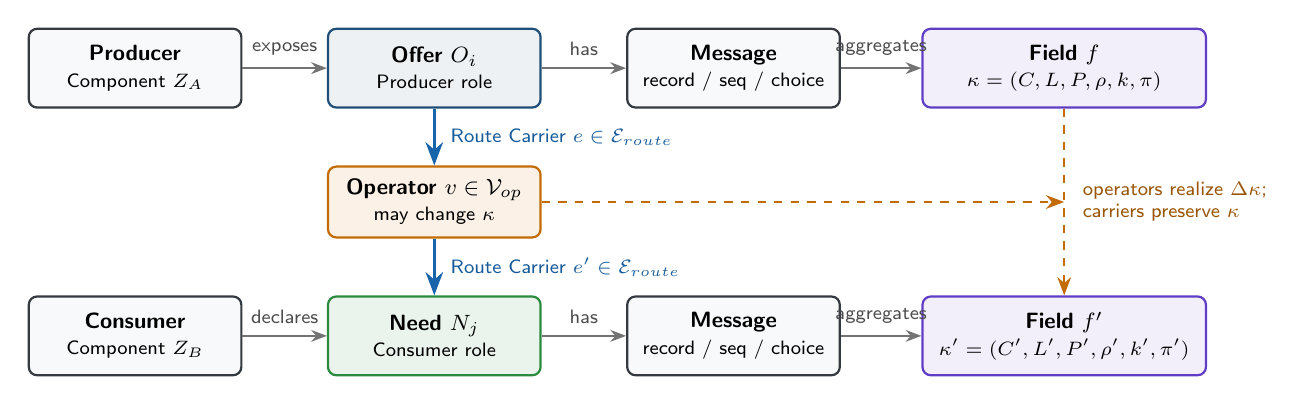
\begin{tikzpicture}[
    >=Stealth,
    font=\footnotesize\sffamily,
    mbox/.style={draw=compBorder, fill=compFill, thick, rounded corners=3pt, minimum width=2.7cm, minimum height=1.0cm, align=center},
    offerbox/.style={draw=techNavy, fill=techNavy!8, thick, rounded corners=3pt, minimum width=2.7cm, minimum height=1.0cm, align=center},
    needbox/.style={draw=boundGreen, fill=boundGreen!10, thick, rounded corners=3pt, minimum width=2.7cm, minimum height=1.0cm, align=center},
    fieldbox/.style={draw=poiPurple, fill=poiPurple!8, thick, rounded corners=3pt, minimum width=3.6cm, minimum height=1.0cm, align=center},
    opbox/.style={draw=accentAmber!90!black, fill=accentAmber!10, thick, rounded corners=3pt, minimum width=2.7cm, minimum height=0.9cm, align=center},
    contains/.style={->, semithick, draw=black!55},
    carrier/.style={->, very thick, draw=fsrBlue},
    opedge/.style={->, thick, dashed, draw=accentAmber!90!black},
    elabel/.style={font=\scriptsize\sffamily, text=black!70}
]
    % Producer row
    \node[mbox] (za) at (0, 1.7) {\textbf{Producer}\\[0pt]{\scriptsize Component $Z_A$}};
    \node[offerbox] (offer) at (3.8, 1.7) {\textbf{Offer $O_i$}\\[0pt]{\scriptsize Producer role}};
    \node[mbox] (msg1) at (7.6, 1.7) {\textbf{Message}\\[0pt]{\scriptsize record / seq / choice}};
    \node[fieldbox] (fld1) at (11.8, 1.7) {\textbf{Field $f$}\\[0pt]{\scriptsize $\kappa = (C, L, P, \rho, k, \pi)$}};

    % Consumer row
    \node[mbox] (zb) at (0, -1.7) {\textbf{Consumer}\\[0pt]{\scriptsize Component $Z_B$}};
    \node[needbox] (need) at (3.8, -1.7) {\textbf{Need $N_j$}\\[0pt]{\scriptsize Consumer role}};
    \node[mbox] (msg2) at (7.6, -1.7) {\textbf{Message}\\[0pt]{\scriptsize record / seq / choice}};
    \node[fieldbox] (fld2) at (11.8, -1.7) {\textbf{Field $f'$}\\[0pt]{\scriptsize $\kappa' = (C', L', P', \rho', k', \pi')$}};

    % Mediation operator between Offer and Need
    \node[opbox] (op) at (3.8, 0) {\textbf{Operator $v \in \mathcal{V}_{\text{op}}$}\\[0pt]{\scriptsize may change $\kappa$}};

    % Containment edges
    \draw[contains] (za) -- node[above=1pt, elabel] {exposes} (offer);
    \draw[contains] (offer) -- node[above=1pt, elabel] {has} (msg1);
    \draw[contains] (msg1) -- node[above=1pt, elabel] {aggregates} (fld1);
    \draw[contains] (zb) -- node[above=1pt, elabel] {declares} (need);
    \draw[contains] (need) -- node[above=1pt, elabel] {has} (msg2);
    \draw[contains] (msg2) -- node[above=1pt, elabel] {aggregates} (fld2);

    % Route carriers (E_route): preserve kappa
    \draw[carrier] (offer.south) -- node[right=2pt, elabel, text=fsrBlue!90!black] {Route Carrier $e \in \mathcal{E}_{\text{route}}$} (op.north);
    \draw[carrier] (op.south) -- node[right=2pt, elabel, text=fsrBlue!90!black] {Route Carrier $e' \in \mathcal{E}_{\text{route}}$} (need.north);

    % Operator effect on Field Colors
    \draw[opedge] (fld1.south) -- node[right=3pt, elabel, text=accentAmber!70!black, align=left] {operators realize $\Delta\kappa$;\\carriers preserve $\kappa$} (fld2.north);
    \draw[opedge] (op.east) -- (11.8, 0);
\end{tikzpicture}%
}
\caption{Metamodel for the Integration Game: Component $\rightarrow$ Offer/Need $\rightarrow$ Message $\rightarrow$ Field typed by Color $\kappa$.  Solid blue edges are Route Carriers ($\mathcal{E}_{\text{route}}$), incurring transport cost $c_{\text{carrier}}$; dashed edges are Mediation Operators ($\mathcal{V}_{\text{op}}$), which may mutate $\kappa$ along one or more of its axes.}
\label{fig:metamodel}
\end{figure}

\paragraph{Color.} A Field is typed by its \emph{Color},
\begin{equation}
    \kappa = (C, L, P, \rho, k, \pi) \in \mathbb{C} \times \mathbb{L} \times \mathbb{P} \times \mathbb{R}_{\text{rep}} \times \mathbb{K} \times \Pi =: \mathcal{K},
    \label{eq:stateful-color}
\end{equation}
where $\mathcal{K}$ denotes the Color space.  Color is distinct from the runtime value $v_{\text{val}}$ it characterizes: a value ranges over a domain determined by $\kappa$, whereas $\kappa$ itself is fixed by the declaration of a port slot.  Color is stateful in three senses:
\begin{itemize}[topsep=2pt, itemsep=1pt, leftmargin=1.8em]
    \item \textbf{Static Coloring $(C, L, P, \rho)$.} $C \in \mathbb{C}$ identifies the Conceptual Entity and its rooted navigational path (e.g., \texttt{Aircraft.sensor.position}).  While the full UDDL standard specifies a rich SQL-like query grammar supporting multi-entity joins and projections, our implementation models $C$ via a simplified canonical semantic paths over CDM entity compositions and observables, which suffices to capture hierarchical $\Delta C$ while keeping conceptual matching decidable and lightweight.  $L \in \mathbb{L}$ is the Logical Frame (measurement system, frame, units), and $P \in \mathbb{P}$ the Platform realization (mirroring the UDDL hierarchy of Section~\ref{sec:bg-uddl}).  $\rho \in \mathbb{R}_{\text{rep}}$ is the in-memory, language-specific realization of the value (e.g., a C \texttt{double}, a CPython \texttt{PyObject*}, a JVM object, or a ROS\,2/DDS language binding).  Note that $\rho$ is not wire serialization, and must be contrasted with the Platform axis $P$, which is the UDDL PDM abstract machine type and precision (e.g., IEEE-754 \texttt{binary64}).  Two ports may align on $(C, L, P)$ (e.g., a WGS84 latitude as \texttt{binary64}) but still differ in $\rho$ (e.g., one has a \texttt{PyObject*} and the other a C-ABI \texttt{double}).  Thus, coupling them directly is unsafe, and a legal move must bind or marshal one realization into the other (Section~\ref{sec:meth-moves}).
    \item \textbf{Kinematics $k$.} $k \in \mathbb{K}$ records the spatiotemporal delivery profile at a boundary port: its topological location $x$ on the board, flow velocity $v$ (an active push flow with $v > 0$ versus a stationary pull potential with $v = 0$), and flow acceleration\footnote{A non-zero $a$ captures impulsive mode transitions, in which a store decelerates a push stream to rest ($a < 0$) or a polling pump accelerates a pull source into a periodic push stream ($a > 0$), while a rate differential $\Delta v$ across a multi-rate boundary dictates downstream buffering and staleness requirements.} $a = \Delta v / \Delta t$, written $k = (x, v, a)$, together with staleness (sample age and its admissible bound).
    \item \textbf{Provenance $\pi$.} $\pi \in \Pi$ records the source lineage and other properties such as assurance level of the Field, and is extended as operators transform it.  For example, a triple modular redundancy (TMR) voter fuses three redundant Fields and emits one whose $\pi$ records the vote history.
\end{itemize}

Luckily, port constraints expressed over $\mathcal{K}$ preserve the algebraic structure of Wymorian coupling.  For a port slot $p$, write $\kappa(p)$ for its Color and $A_{\kappa(p)}$ for the alphabet of values it admits; $A_{\kappa(p)}$ is determined by the projection $(C, L, P, \rho)$, while $k$ and $\pi$ constrain admissible delivery timing and lineage.  A \emph{Play} $\mathcal{P}$ is a candidate integration on the board; composition of its components induces the \emph{Coupled Resultant} $Z_b = \mathrm{RSY}(\mathcal{P})$.

\begin{proposition}[Color Typed Compatibility] \label{prop:wymore-iso}
Let $TYR$ be a catalog of discrete component systems and Mediation Operators whose ports are partitioned into elementary Field slots, and let $\kappa$ assign a Color $\kappa(p) \in \mathcal{K}$ to each slot $p$.  Define the color-refined Technology Catalog $TYR_{\mathcal{K}}$ by restricting the alphabet of each slot to $A_{\kappa(p)}$.  Then a Play $\mathcal{P}$ is legal (i.e., every wired port pair $(p_{\text{out}}, p_{\text{in}})$ satisfies $\mathrm{proj}_{CL P\rho}(\kappa(p_{\text{out}})) = \mathrm{proj}_{CL P\rho}(\kappa(p_{\text{in}}))$, the kinematics $k(p_{\text{out}})$ are admissible for $k(p_{\text{in}})$, and $\pi(p_{\text{out}})$ meets the provenance predicate of $p_{\text{in}}$) if and only if $\mathcal{P}$ forms a valid Wymorian System Coupling Recipe $SCR = (VSCR, CSCR)$ over $TYR_{\mathcal{K}}$ whose wired pairs additionally satisfy these kinematic and provenance admissibility conditions.  In that case $A_{\kappa(p_{\text{out}})} = A_{\kappa(p_{\text{in}})}$ for every pair in $CSCR$, and synchronous composition induces a unique Coupled Resultant discrete system $Z_b = \mathrm{RSY}(SCR) \in \mathrm{CTL}(TYR_{\mathcal{K}})$.
\end{proposition}

\begin{proof}[Proof Sketch]
In T3SD, an $SCR = (VSCR, CSCR)$ is well-formed iff $CSCR$ is a bijection between a subset of component output ports and a subset of component input ports such that the output alphabet of each source port equals the input alphabet of its destination~\cite{Wymore1993}.  Because $A_{\kappa(p)}$ is a function of the projection $(C, L, P, \rho)$ of $\kappa(p)$, equality of these projections implies $A_{\kappa(p_{\text{out}})} = A_{\kappa(p_{\text{in}})}$ and, up to declared equivalence of Colors, conversely.  In particular, two ports that agree on $(C, L, P)$ but differ in $\rho$ have distinct alphabets, so their direct coupling is not a well-formed $CSCR$ edge; this is the formal counterpart of the unsafe \texttt{PyObject*}/C-ABI couple above.  The axes $k$ and $\pi$ do not change alphabets but gate coupling: they restrict wiring to pairs whose delivery profile and lineage satisfy the Need's declared predicates, and are discharged as the Tier~1 and Tier~2 conditions of Section~\ref{sec:meth-winning}.  Route Carriers in $\mathcal{E}_{\text{route}}$ connect ports of identical Color and therefore are edges of $CSCR$ rather than members of $VSCR$.  Any Color discrepancy $\Delta\kappa$ between an Offer and a Need must be resolved by an interior Mediation Operator $v \in \mathcal{V}_{\text{op}} \subseteq VSCR$ whose input port has alphabet $A_{\kappa_{\text{in}}}$ and whose output port has alphabet $A_{\kappa_{\text{out}}}$.  The step transition $\delta_b$ and readout $\rho_{\text{out},b}$ of $Z_b = \mathrm{RSY}(SCR)$ then follow from the standard Wymorian coupling algebra.
\end{proof}

\subsection{Mediation Operators and Legal Moves} \label{sec:meth-moves}

Mediation Operators in $TYR_{\mathcal{K}}$ are organized into four families (Table~\ref{tab:legal-moves}):

\begin{enumerate}[topsep=2pt, itemsep=1pt, leftmargin=1.8em]
    \item \textbf{Stateful Recoloring:} Operators that transform a Field along one or more axes of $\kappa$.  A \emph{Conceptual Recolor} ($\Delta C$) maps a Field between equivalent or related CDM concepts; a \emph{Logical Recolor} ($\Delta L$) converts units, reference frames, or coordinate systems via a declared quantitative transformation; a \emph{Platform Recolor} ($\Delta P$) widens, narrows, or repacks data types across PDM encodings; and a \emph{Runtime Representation Binding/Marshaling} operator ($\Delta\rho$) re-expresses the same value in a different in-memory or language-runtime realization (foreign function interfaces, JNI bridges, language-binding conversions, etc.).
    \item \textbf{Structural Aggregation:} Because Messages are containers of Fields, \emph{Assemble} and \emph{Disassemble} operators pack constituent Fields into composite Messages or split Messages into individual Fields, while \emph{Project} and \emph{Inject} select subsets of Field slots or insert constant or derived Fields, preserving Colors.
    \item \textbf{Computational Derivation and Filtering:} \emph{Derive} is the general multi-input synthesis operator: it consumes $N \ge 1$ Fields (potentially correlated from distinct Offers) and computes $M \ge 1$ output Fields with declared target Colors (for example, combining host vehicle position, attitude quaternion, and lever-arm geometry to derive sensor position, executing a state-estimation filter update).  \emph{Filter/Validate} forwards or suppresses Messages based on deterministic predicates over payload values or provenance.
    \item \textbf{Topology, Storage, and Flow Mediation:} Operators that mutate kinematics $k$ and interaction topology while leaving $(C, L, P, \rho)$ invariant.  \emph{Fan-Out}, \emph{Fan-In}, and \emph{Temporal Join} alter routing multiplicity and correlate asynchronous Messages across bounded time windows; \emph{Stores} (latest-value latches, bounded FIFO queues, or keyed maps) introduce internal memory state; \emph{Mode Bridges} reconcile mismatched push/pull transfer mechanics; and \emph{Temporal Control} operators enforce data freshness via stale-age gates and failover multiplexers.
\end{enumerate}

\begin{table}[t]
\centering
\caption{Taxonomy of Mediation Operator families and their effects on Color $\kappa = (C, L, P, \rho, k, \pi)$.}
\label{tab:legal-moves}
\footnotesize
\begin{tabularx}{\linewidth}{@{}>{\raggedright\arraybackslash}p{2.7cm} >{\raggedright\arraybackslash}p{2.8cm} >{\raggedright\arraybackslash}p{3.1cm} >{\raggedright\arraybackslash}X@{}}
\toprule
\textbf{Move Family} & \textbf{Mediation Operators} & \textbf{Color Effect} & \textbf{Kinematic \& State Effect in $Z_b = \mathrm{RSY}(\mathcal{P})$} \\
\midrule
Stateful Recoloring & Conceptual, Logical, Platform, Runtime Binding/Marshaling & Modifies $C$, $L$, $P$ ($\Delta C$, $\Delta L$, $\Delta P$) or realization $\rho$ ($\Delta\rho$, with $(C, L, P)$ invariant) & Stateless synchronous value or realization transformation; tracks precision narrowing. \\
\addlinespace[2pt]
Structural Aggregation & Assemble, Disassemble, Project, Inject & Preserves $\kappa$ of constituent Fields & Repackages Field slots between Producer and Consumer Message structures. \\
\addlinespace[2pt]
Derivation \& Filtering & Derive / Synthesize, Filter / Validate & Produces declared target $\kappa_{\text{out}}$ (extends lineage $\pi$) & Fuses $N$ inputs into $M$ derived Fields or suppresses invalid or out-of-bounds samples. \\
\addlinespace[2pt]
Flow, Storage \& Time & Fan/Join, Store, Mode Bridge, Stale Gate & Invariant in $(C, L, P, \rho)$; modifies only $k$ & Introduces internal state $S$, decouples push/pull kinematics, and enforces freshness bounds. \\
\bottomrule
\end{tabularx}
\end{table}

\begin{figure}[t]
\centering
\resizebox{\linewidth}{!}{%
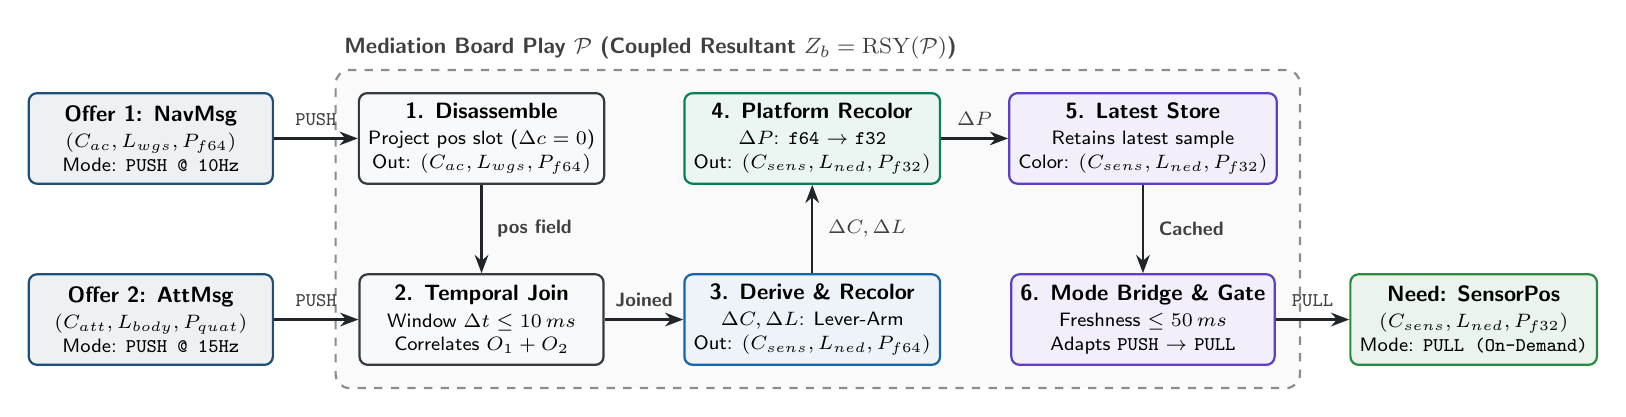
\begin{tikzpicture}[
    >=Stealth,
    font=\footnotesize\sffamily,
    offerbox/.style={draw=techNavy, fill=techNavy!8, thick, rounded corners=3pt, minimum width=3.1cm, minimum height=1.15cm, align=center},
    needbox/.style={draw=boundGreen, fill=boundGreen!10, thick, rounded corners=3pt, minimum width=3.1cm, minimum height=1.15cm, align=center},
    opbox/.style={draw=compBorder, fill=compFill, thick, rounded corners=3pt, minimum width=3.1cm, minimum height=1.15cm, align=center},
    storebox/.style={draw=poiPurple, fill=poiPurple!8, thick, rounded corners=3pt, minimum width=3.1cm, minimum height=1.15cm, align=center},
    route/.style={->, thick, draw=wireInk},
    clabel/.style={font=\scriptsize\sffamily\bfseries, text=black!75}
]
    % Producer Offers (Left Boundary, x = 0)
    \node[offerbox] (o1) at (0, 1.15) {
        \textbf{Offer 1: NavMsg}\\[0pt]
        {\scriptsize $(C_{\text{ac}}, L_{\text{wgs}}, P_{\text{f64}})$}\\[-1pt]
        {\scriptsize Mode: \texttt{PUSH @ 10Hz}}
    };
    \node[offerbox] (o2) at (0, -1.15) {
        \textbf{Offer 2: AttMsg}\\[0pt]
        {\scriptsize $(C_{\text{att}}, L_{\text{body}}, P_{\text{quat}})$}\\[-1pt]
        {\scriptsize Mode: \texttt{PUSH @ 15Hz}}
    };

    % Interior Board Column 1 (x = 4.2)
    \node[opbox] (dis) at (4.2, 1.15) {
        \textbf{1. Disassemble}\\[0pt]
        {\scriptsize Project pos slot ($\Delta c = 0$)}\\[-1pt]
        {\scriptsize Out: $(C_{\text{ac}}, L_{\text{wgs}}, P_{\text{f64}})$}
    };
    \node[opbox] (join) at (4.2, -1.15) {
        \textbf{2. Temporal Join}\\[0pt]
        {\scriptsize Window $\Delta t \le 10\,\text{ms}$}\\[-1pt]
        {\scriptsize Correlates $O_1 + O_2$}
    };

    % Interior Board Column 2 (x = 8.4)
    \node[opbox, fill=fsrBlue!8, draw=fsrBlue] (der) at (8.4, -1.15) {
        \textbf{3. Derive \& Recolor}\\[0pt]
        {\scriptsize $\Delta C, \Delta L$: Lever-Arm}\\[-1pt]
        {\scriptsize Out: $(C_{\text{sens}}, L_{\text{ned}}, P_{\text{f64}})$}
    };
    \node[opbox, fill=bsrTeal!8, draw=bsrTeal] (prec) at (8.4, 1.15) {
        \textbf{4. Platform Recolor}\\[0pt]
        {\scriptsize $\Delta P$: \texttt{f64} $\to$ \texttt{f32}}\\[-1pt]
        {\scriptsize Out: $(C_{\text{sens}}, L_{\text{ned}}, P_{\text{f32}})$}
    };

    % Interior Board Column 3 (x = 12.6)
    \node[storebox] (store) at (12.6, 1.15) {
        \textbf{5. Latest Store}\\[0pt]
        {\scriptsize Retains latest sample}\\[-1pt]
        {\scriptsize Color: $(C_{\text{sens}}, L_{\text{ned}}, P_{\text{f32}})$}
    };
    \node[storebox] (gate) at (12.6, -1.15) {
        \textbf{6. Mode Bridge \& Gate}\\[0pt]
        {\scriptsize Freshness $\le 50\,\text{ms}$}\\[-1pt]
        {\scriptsize Adapts \texttt{PUSH} $\to$ \texttt{PULL}}
    };

    % Consumer Need (Right Boundary, x = 16.8)
    \node[needbox] (need) at (16.8, -1.15) {
        \textbf{Need: SensorPos}\\[0pt]
        {\scriptsize $(C_{\text{sens}}, L_{\text{ned}}, P_{\text{f32}})$}\\[-1pt]
        {\scriptsize Mode: \texttt{PULL (On-Demand)}}
    };

    % Routes
    \draw[route] (o1) -- node[above=1pt, clabel] {\texttt{PUSH}} (dis);
    \draw[route] (o2) -- node[above=1pt, clabel] {\texttt{PUSH}} (join);
    \draw[route] (dis) -- node[right=2pt, clabel] {pos field} (join);
    \draw[route] (join) -- node[above=1pt, clabel] {Joined} (der);
    \draw[route] (der) -- node[right=2pt, clabel] {$\Delta C, \Delta L$} (prec);
    \draw[route] (prec) -- node[above=1pt, clabel] {$\Delta P$} (store);
    \draw[route] (store) -- node[right=2pt, clabel] {Cached} (gate);
    \draw[route] (gate) -- node[above=1pt, clabel] {\texttt{PULL}} (need);

    % Background Board Frame
    \begin{scope}[on background layer]
        \node[draw=black!45, dashed, thick, fill=black!2, rounded corners=5pt, fit=(dis)(join)(der)(prec)(store)(gate), inner sep=8pt,
              label={[anchor=south west, font=\footnotesize\sffamily\bfseries, text=black!75]north west:Mediation Board Play $\mathcal{P}$ (Coupled Resultant $Z_b = \mathrm{RSY}(\mathcal{P})$)}] {};
    \end{scope}
\end{tikzpicture}%
}
\caption{An example Play $\mathcal{P}$ on a Mediation Board.  Two asynchronous push-mode Producer Offers are disassembled, temporally joined, transformed across conceptual and logical axes via a lever-arm derivation, narrowed in platform precision, and buffered in a latest-value store with a freshness-gated mode bridge to satisfy a pull-mode Consumer Need.  Operator boxes display the $(C, L, P)$ projection of each Field's Color $\kappa$ for brevity; $\rho$, $k$, and $\pi$ are carried along and mutate only where an operator (e.g., the Store and Mode Bridge, which alter $k$) is applied.}
\label{fig:mediation-board}
\end{figure}

Figure~\ref{fig:mediation-board} illustrates how a Play $\mathcal{P}$ composes these operator families to resolve both $(C, L, P)$ differences and the push-to-pull kinematic gap between two Producer Offers and a Consumer Need.

\subsection{Behavioral Contracts} \label{sec:meth-contracts}

Typing alone does not establish that a Coupled Resultant behaves correctly or as desired over time.  We encode behavioral requirements as Input/Output Requirements $IOR = (OLR, IR, ITR, OR, OTR, ER)$, where the operational life requirement satisfies $OLR \in \mathbb{N}^+ \cup \{\infty\}$ and induces the timescale $TSR(IOR) = \{t \in \mathbb{N} \mid t < OLR\}$.  When $OLR = \infty$, $TSR = \mathbb{N}$.  To encode $IOR$s without loss of generality, we use a Universal Live Sequence Chart (uLSC) fragment over two boundary lifelines: the external environment ($\mathsf{Env}$) and the system ($\mathsf{Sys}$).

\begin{definition}[Universal Live Sequence Chart (uLSC)] \label{def:ulsc}
A uLSC over input alphabet $IR$ and output alphabet $OR$ is a tuple $\mathcal{L} = (\tau, \mathcal{P}_{\text{in}}, \mathcal{A}_{\text{out}})$, where $\tau \subseteq \mathbb{N}$ is the discrete operational horizon (finite, or $\tau = \mathbb{N}$ when $OLR = \infty$), $\mathcal{P}_{\text{in}} \subseteq IR^{\mathbb{N}}$ is the \emph{cold Pre-Chart} predicate specifying the set of eligible environmental input trajectories that activate the contract, and $\mathcal{A}_{\text{out}} : IR^{\mathbb{N}} \times OR^{\mathbb{N}} \to \{\mathrm{true}, \mathrm{false}\}$ is the \emph{hot Main-Chart} relation over $\omega$-trajectories, specifying admissible input--output trajectory pairs (including value tolerances, delivery deadlines, and quiet-output \emph{silence} obligations).
\end{definition}

A discrete system $Z = (S, IR, OR, \delta, \rho_{\text{out}})$ initialized at $s_0 \in S$ \emph{satisfies} a uLSC $\mathcal{L}$ on timescale $T \subseteq \tau$ ($T \neq \emptyset$), written $(Z, s_0) \models_T \mathcal{L}$, when every Pre-Chart activation forces a Main-Chart fulfillment:
\begin{equation}
\begin{aligned}
    (Z, s_0) \models_T \mathcal{L}
    \iff{}&
    \forall f \in \mathcal{P}_{\text{in}},\; \forall h \in IR^{\mathbb{N}},\\
    &\quad\big(\forall t \in \tau,\; h(t) = f(t)\big) \implies \exists g \in OR^{\mathbb{N}},\; \mathcal{A}_{\text{out}}(f, g) \wedge \big(\forall t \in T,\; y_Z(s_0, h)(t) = g(t)\big).
\end{aligned}
    \label{eq:lsc-sat}
\end{equation}
We write $\mathrm{CTL}(\mathcal{L})$ for the set of all triples $(Z, s_0, T)$ such that $(Z, s_0) \models_T \mathcal{L}$.  If an input trajectory $h$ fails to match $\mathcal{P}_{\text{in}}$ on $\tau$, the cold Pre-Chart is vacated without penalty; conversely, if the Pre-Chart matches on $\tau$ but no allowed output trajectory $g$ agrees with $y_Z(s_0, h)$ on $T$, a \emph{Hot Breach} occurs, written $(Z, s_0, f) \not\models_T \mathcal{L}$ for the activating scenario $f \in \mathcal{P}_{\text{in}}$.  Given any Wymorian Input/Output Requirement $IOR$, its \emph{characteristic uLSC} $\mathcal{L}(IOR)$ is constructed by setting $\tau = TSR(IOR)$, $\mathcal{P}_{\text{in}} = ITR$, and $\mathcal{A}_{\text{out}}(f, g) \Longleftrightarrow g \in ER(f)$ (Fig.~\ref{fig:ulsc-diagram}).  Because $OLR \in \mathbb{N}^+ \cup \{\infty\}$, this construction covers both finite horizons and the infinite horizon $\tau = TSR = \mathbb{N}$, in which $\mathcal{P}_{\text{in}} \subseteq IR^{\mathbb{N}}$ and $\mathcal{A}_{\text{out}}$ range over $\omega$-trajectories.

\begin{theorem}[Correspondence Between $IOR$s and uLSCs] \label{thm:ior-lsc}
For every Input/Output Requirement $IOR = (OLR, IR, ITR, OR, OTR, ER)$ with $OLR \in \mathbb{N}^+ \cup \{\infty\}$, discrete system $Z = (S, IR, OR, \delta, \rho_{\text{out}})$, initial state $s_0 \in S$, and nonempty evaluation timescale $T \subseteq TSR(IOR)$,
\begin{equation}
    (Z, s_0) \models_T \mathcal{L}(IOR)
    \iff (Z, s_0) \models_T IOR
    \iff (Z, s_0, T) \in \mathrm{CTL}(IOR).
    \label{eq:ior-lsc-equiv}
\end{equation}
Consequently $\mathrm{CTL}(\mathcal{L}(IOR)) = \mathrm{CTL}(IOR)$.  In particular, the equivalence holds in the infinite case $OLR = \infty$, $TSR = \mathbb{N}$, $T = \mathbb{N}$.  Moreover, a Hot Breach occurs on an input scenario $f \in ITR$ (with extension $h$ agreeing with $f$ on $TSR$) if and only if $(Z, s_0, f) \not\models_T IOR$.
\end{theorem}

\begin{proof}[Proof Sketch]
By definition of $\mathcal{L}(IOR)$, $\tau = TSR(IOR)$, $\mathcal{P}_{\text{in}} = ITR$, and $\mathcal{A}_{\text{out}}(f, g) \iff g \in ER(f)$.  Substituting these directly into~\eqref{eq:lsc-sat} yields the exact trajectory quantification of $(Z, s_0) \models_T IOR$ from Section~\ref{sec:bg-t3sd}: $T \neq \emptyset$, $T \subseteq TSR(IOR)$, and for every $f \in ITR$ and extension $h$ agreeing with $f$ on $TSR(IOR)$, there exists $g \in ER(f)$ matching $y_Z(s_0, h)(t)$ at all $t \in T$.  Membership $(Z, s_0, T) \in \mathrm{CTL}(IOR)$ is synonymous with that quantification, so the three sides of~\eqref{eq:ior-lsc-equiv} coincide and $\mathrm{CTL}(\mathcal{L}(IOR)) = \mathrm{CTL}(IOR)$.  The argument is syntactic and never uses finiteness of $\tau$ or $T$, so it covers the infinite case: when $OLR = \infty$ we have $\tau = \mathbb{N}$, the agreement condition $\forall t \in \tau,\, h(t) = f(t)$ forces $h = f$, $g \in ER(f) \subseteq OR^{\mathbb{N}}$ ranges over entire $\omega$-trajectories, and the universal quantifier over $t \in T = \mathbb{N}$ is carried identically on both sides of~\eqref{eq:ior-lsc-equiv}.  Defining $\mathcal{A}_{\text{out}}$ via full envelope membership $g \in ER(f)$ is essential: a pointwise projection requiring only $y_Z(s_0, h)(t) \in \{g(t) \mid g \in ER(f)\}$ at each tick $t$ independently is strictly weaker whenever $ER(f)$ couples outputs across ticks.  Negating~\eqref{eq:lsc-sat} immediately yields the Hot Breach condition $(Z, s_0, f) \not\models_T \mathcal{L}$.
\end{proof}

\begin{figure}[t]
\centering
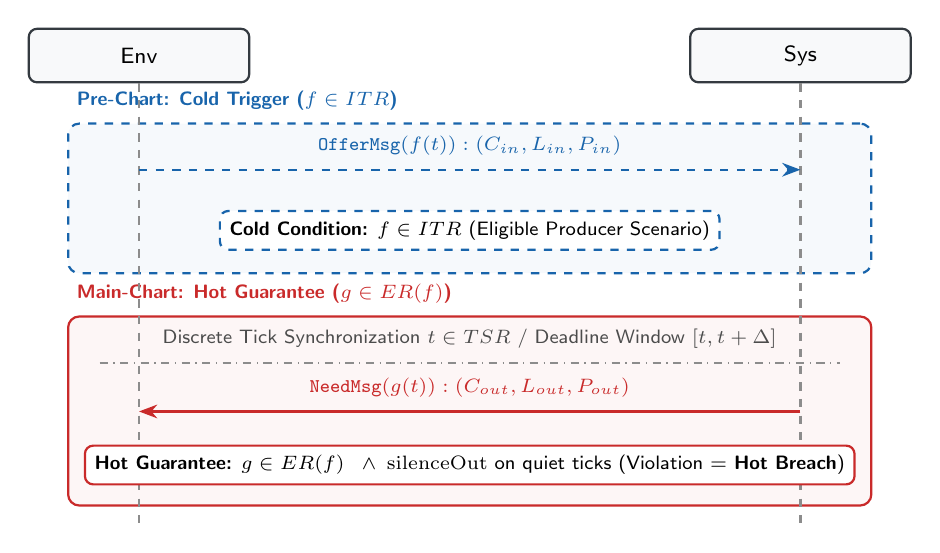
\begin{tikzpicture}[
    >=Stealth,
    font=\footnotesize\sffamily,
    lifelinehead/.style={draw=compBorder, fill=compFill, thick, rounded corners=3pt, minimum width=2.8cm, minimum height=0.68cm, align=center, font=\footnotesize\sffamily\bfseries},
    coldframe/.style={draw=coldBlue, dashed, thick, fill=coldBlue!4, rounded corners=4pt},
    hotframe/.style={draw=hotRed, solid, thick, fill=hotRed!4, rounded corners=4pt},
    lsccond/.style={draw=black!30, fill=white, rounded corners=3pt, font=\scriptsize\sffamily, inner sep=3.5pt, align=center}
]
    % Lifeline Heads
    \node[lifelinehead] (env) at (0, 0) {$\mathsf{Env}$};
    \node[lifelinehead] (sys) at (8.4, 0) {$\mathsf{Sys}$};

    % Pre-Chart (Cold Trigger Region): y from -0.85 to -2.75
    \node[coldframe, minimum width=10.2cm, minimum height=1.90cm, anchor=north] (pre_box) at (4.2, -0.85) {};
    \node[font=\scriptsize\sffamily\bfseries, text=coldBlue, anchor=south west] at ([yshift=1pt]pre_box.north west)
      {Pre-Chart: Cold Trigger ($f \in ITR$)};

    % Main-Chart (Hot Guarantee Region): y from -3.30 to -5.70
    \node[hotframe, minimum width=10.2cm, minimum height=2.40cm, anchor=north] (main_box) at (4.2, -3.30) {};
    \node[font=\scriptsize\sffamily\bfseries, text=hotRed, anchor=south west] at ([yshift=1pt]main_box.north west)
      {Main-Chart: Hot Guarantee ($g \in ER(f)$)};

    % Vertical Lifeline Rays
    \draw[dashed, thick, black!45] (env.south) -- (0, -5.95);
    \draw[dashed, thick, black!45] (sys.south) -- (8.4, -5.95);

    % Cold Input Message (Env -> Sys)
    \draw[-{Stealth}, dashed, thick, draw=coldBlue] (0, -1.45) --
      node[above=1.5pt, font=\scriptsize\sffamily, text=coldBlue] {\texttt{OfferMsg}$(f(t)) : (C_{\text{in}}, L_{\text{in}}, P_{\text{in}})$} (8.4, -1.45);

    % Cold Guard Condition
    \node[lsccond, draw=coldBlue, dashed, thick] at (4.2, -2.22)
      {\textbf{Cold Condition:} $f \in ITR$ (Eligible Producer Scenario)};

    % Tick Synchronization
    \draw[dashdotted, thick, black!45] (-0.5, -3.90) --
      node[above=1.5pt, font=\scriptsize\sffamily, text=black!70] {Discrete Tick Synchronization $t \in TSR$ / Deadline Window $[t, t+\Delta]$} (8.9, -3.90);

    % Hot Output Message (Sys -> Env)
    \draw[-{Stealth}, solid, thick, draw=hotRed] (8.4, -4.52) --
      node[above=1.5pt, font=\scriptsize\sffamily, text=hotRed] {\texttt{NeedMsg}$(g(t)) : (C_{\text{out}}, L_{\text{out}}, P_{\text{out}})$} (0, -4.52);

    % Hot Envelope Condition
    \node[lsccond, draw=hotRed, solid, thick] at (4.2, -5.20)
      {\textbf{Hot Guarantee:} $g \in ER(f)$ \enspace$\wedge$\enspace $\mathrm{silenceOut}$ on quiet ticks (Violation $=$ \textbf{Hot Breach})};
\end{tikzpicture}
\caption{Diagrammatic structure of the characteristic uLSC $\mathcal{L}(IOR)$.  A match on the dashed blue Cold Pre-Chart triggers the solid red Hot Main-Chart obligation; any violation of the output value envelope, timing window, or silence constraint induces a Hot Breach.}
\label{fig:ulsc-diagram}
\end{figure}

\subsection{Winning Conditions} \label{sec:meth-winning}

We evaluate a candidate Play $\mathcal{P}$ across three tiers:
\begin{enumerate}[label=\textbf{Tier \arabic*}, leftmargin=3.4em, topsep=2pt, itemsep=1pt]
    \item \textbf{(Static Stateful-Color and Structural Compatibility):} For every required Field slot in every Consumer Need $N_j \in \mathcal{N}$, there exists a directed path through $\mathcal{P}$ originating at one or more Producer Offers $O_i \in \mathcal{O}$ along which only legal Mediation Operators are applied, Message aggregations assemble with matching slot structures, and the terminal Field's Color $\kappa$ matches the required $\kappa_{N_j}$: $(C, L, P, \rho)$ agree with $(C_{N_j}, L_{N_j}, P_{N_j}, \rho_{N_j})$, and $\pi$ satisfies the provenance predicate $\pi_{N_j}$.
    \item \textbf{(Flow and Kinematic Compatibility):} Along every route in $\mathcal{P}$, the kinematic component $k$ is mutually compatible (every push output connects to a push-capable input, and every pull input connects to a pull-capable output, or a Mode Bridge mediates the transition), staleness/freshness bounds are met by operator and Route Carrier latencies, all storage capacities are strictly positive, and all temporal operators share a consistent time base.
    \item \textbf{(Behavioral Satisfaction):} Let $Z_b = \mathrm{RSY}(\mathcal{P})$ be the Coupled Resultant induced by the Play.  Given the problem's $IOR$ and its characteristic uLSC $\mathcal{L}(IOR)$ (Definition~\ref{def:ulsc}), the Coupled Resultant satisfies the behavioral contract over the declared operational horizon without a Hot Breach:
    \[
        (Z_b, s_0) \models_{TSR} \mathcal{L}(IOR).
    \]
    By Theorem~\ref{thm:ior-lsc} this is equivalent to $(Z_b, s_0) \models_{TSR} IOR$ and to $(Z_b, s_0, TSR) \in \mathrm{CTL}(IOR)$, including for $OLR = \infty$.
\end{enumerate}

A Play $\mathcal{P}$ \emph{wins} the Integration Game if and only if it satisfies Tiers~1, 2, and~3 simultaneously.  By Proposition~\ref{prop:wymore-iso} and Theorem~\ref{thm:ior-lsc}, a winning Play constitutes a well-formed Color-typed coupling recipe over $TYR_{\mathcal{K}}$ whose Coupled Resultant obeys $(Z_b, s_0) \models_{TSR} \mathcal{L}(IOR)$ over the verified trajectory suite $ITR_{\text{test}} \subseteq ITR$, and across all admissible trajectories within any symbolically certified contract fragment (Section~\ref{sec:meth-rl}).

\subsection{Cost Functional and Trade-Offs} \label{sec:meth-cost}

Winning Plays can still differ dramatically in footprint, latency, and fidelity.  We therefore define an Integration Cost Functional $\mathcal{J}(\mathcal{P})$ that both supports Wymorian $CR$/$PR$/$TR$ trade offs and supplies guidance for RL: frontier potential $\mathcal{J}_{\text{tier1,2}}$ guides assembly of sparse valid graphs (Tiers~1--2), $C_{\text{breach}}$ is a temporal/value guide over traces (Tier~3), $C_{\text{static}}$ versus $C_{\text{dyn}}$ mirrors design-time Cost Requirements versus runtime Performance Requirements, and the piecewise fitness $\mathcal{S}$ preserves exact cost differences among feasible Plays while compressing $\Omega$-scale penalties without saturating gradients.

\begin{enumerate}[topsep=2pt, itemsep=1pt, leftmargin=1.8em]
    \item \textbf{Static Construction Cost $C_{\text{static}}(\mathcal{P})$ ($CR$):} Quantifies the structural and resource footprint of the Mediation Board:
    \begin{equation}
        C_{\text{static}}(\mathcal{P}) = \sum_{v \in \mathcal{V}_{\text{op}}} c_{\text{op}}(v) + \sum_{s \in \mathcal{V}_{\text{store}}} c_{\text{mem}}(\mathrm{cap}_s, \mathrm{ret}_s) + \sum_{r \in \mathcal{E}_{\text{route}}} c_{\text{carrier}}(r),
        \label{eq:c-static}
    \end{equation}
    where $\mathcal{V}_{\text{store}} \subseteq \mathcal{V}_{\text{op}}$ are the Store operators.  In general, $(c_{\text{op}}, c_{\text{mem}}, c_{\text{carrier}})$ are normalized non-negative resource weights derived from target-platform profiling or catalog specifications (e.g., WCET/FLOPs per invocation for $c_{\text{op}}$, allocated buffer bytes $\times$ retention ticks for $c_{\text{mem}}$, and bus bandwidth or IPC marshaling overhead for $c_{\text{carrier}}$).  In our implementation, operators are assigned $c_{\text{op}}$ by family: stateless recoloring/projection in $[0.1, 0.3]$, stateful stores/bridges in $[0.3, 0.5]$ plus $c_{\text{mem}}$ proportional to capacity, and multi-input derivations or heavy batch solvers in $[0.5, 1.5]$.

    \item \textbf{Dynamic Operational Cost $C_{\text{dyn}}(\mathcal{P}, f)$ ($PR$):} Quantifies trajectory-level quality-of-service degradation over an input scenario $f \in ITR$ across time $t \in TSR$ (with temporal discount factor $\gamma \in (0, 1]$):
    \begin{equation}
        C_{\text{dyn}}(\mathcal{P}, f) = \sum_{t \in TSR} \gamma^t \Big[ w_{\text{lat}}\,\mathrm{Latency}(t) + w_{\text{loss}}\,\mathrm{InfoLoss}(t) + w_{\text{drop}}\,\mathbf{1}_{\{\mathrm{Code}(t) \neq \mathsf{Success}\}} \Big],
        \label{eq:c-dyn}
    \end{equation}
    capturing end-to-end transport latency, precision loss from narrowing platform conversions, and runtime flow disruptions (e.g., stale sample drops).

    \item \textbf{Behavioral Breach Penalty $C_{\text{breach}}(\mathcal{P}, f)$:} Quantifies departure from the required behavioral envelope $ER(f)$:
    \begin{equation}
        C_{\text{breach}}(\mathcal{P}, f) = \Omega \cdot \mathbf{1}_{\mathsf{HotBreach}}(\mathcal{P}, f) + \sum_{t \in TSR} \inf_{g \in ER(f)} d_{\text{val}}\big(y_{Z_b}(t),\, g(t)\big),
        \label{eq:c-breach}
    \end{equation}
    where $\Omega > 0$ is a categorical breach margin triggered upon any uLSC Hot Breach, and $d_{\text{val}}$ is a continuous distance metric measuring how far the generated output $y_{Z_b}(t)$ deviates from the admissible envelope $ER(f)$.
\end{enumerate}

Combining these terms with the structural and kinematic frontier potentials over a distribution of operational scenarios $\mathcal{D}(ITR)$ yields the composite Integration Cost Functional:
\begin{equation}
    \mathcal{J}(\mathcal{P}) = \mathcal{J}_{\text{tier1,2}}(\mathcal{P}) + C_{\text{static}}(\mathcal{P}) + \mathbb{E}_{f \sim \mathcal{D}(ITR)}\!\Big[ C_{\text{dyn}}(\mathcal{P}, f) + C_{\text{breach}}(\mathcal{P}, f) \Big],
    \label{eq:j-total}
\end{equation}
where $\mathcal{J}_{\text{tier1,2}} = \mathcal{J}_{\text{tier1}} + \mathcal{J}_{\text{tier2}}$ is the open-frontier potential, defined explicitly as
\begin{equation}
    \mathcal{J}_{\text{tier1,2}}(\mathcal{P}) = \sum_{N_j \in \mathcal{N}_{\text{open}}(\mathcal{P})} \Big( w_{\text{unconnected}} + \min_{O \in \mathcal{F}_{\text{live}}(\mathcal{P})} \Delta_{\kappa}(O, N_j) \Big).
    \label{eq:j-frontier}
\end{equation}
Here $\mathcal{N}_{\text{open}}(\mathcal{P}) \subseteq \mathcal{N}$ is the set of Needs not yet satisfied at Tiers~1 and~2, $\mathcal{F}_{\text{live}}(\mathcal{P})$ is the \emph{live offer frontier} (i.e., the set of Offers reachable via directed paths from boundary Producers) and $w_{\text{unconnected}}$ is an open-port penalty.  The term $\Delta_{\kappa}(O, N_j)$ is the \emph{Color distance}: the sum $\Delta_{\text{tier1}} + \Delta_{\text{tier2}}$ of a Tier~1 distance over the axes $(C, L, P, \rho, \pi)$ and a Tier~2 kinematic mismatch over $k$.  By convention the minimum over an empty frontier equals a fixed maximal distance $\Delta_{\max}$.  Tier~3 contributes to $\mathcal{J}$ only through $C_{\text{breach}}$ and is \emph{not} a frontier term.

\paragraph{Fitness.} The fitness $\mathcal{S}(\mathcal{P})$ is a strictly decreasing, $C^1$-smooth map of a soft cost $\mathrm{softJ}(\mathcal{P}) = \mathcal{J}(\mathcal{P}) / J_{\text{ref}}$ (the cost $\mathcal{J}$ normalized by a fixed reference scale $J_{\text{ref}} > 0$) into $(0, S_{\max}]$, with a piecewise form that is linear up to a knee $x_k \in (0, S_{\max})$ and rational beyond it:
\begin{equation}
    \mathcal{S}(\mathcal{P}) = \sigma\big(\mathrm{softJ}(\mathcal{P})\big), \qquad
    \sigma(x) =
    \begin{cases}
        S_{\max} - x, & 0 \le x \le x_k, \\[3pt]
        \dfrac{(S_{\max} - x_k)^2}{x + S_{\max} - 2x_k}, & x > x_k.
    \end{cases}
    \label{eq:fitness-S}
\end{equation}
The two branches agree in value ($S_{\max} - x_k$) and slope ($-1$) at $x = x_k$, so $\sigma$ is $C^1$, strictly decreasing, and bounded below by $0$ without ever reaching it; fitness therefore preserves a nonvanishing gradient across arbitrarily poor candidates.

To guarantee that $\mathcal{J}(\mathcal{P})$ induces a well-posed value ordering over candidate architectures, we desire that it aligns with some expectations we have about such a cost functional should behave.  To capture these intuitive expectations, we define seven axioms:
\begin{enumerate}[label=\textbf{(A\arabic*)}, leftmargin=2.4em, topsep=2pt, itemsep=1pt]
    \item \textbf{Feasibility Dominance:} Every winning Play ($\mathcal{J}_{\text{tier1,2}}=C_{\text{breach}}=0$) achieves strictly lower cost $\mathcal{J}$ and strictly higher fitness $\mathcal{S}$ than any losing Play.
    \item \textbf{Only Count Connected Moves:} Placing an interior Mediation Operator disconnected from Producers leaves $\mathcal{F}_{\text{live}}(\mathcal{P})$ unchanged and strictly increases $\mathcal{J}$ by $c_{\text{op}}(v) > 0$.
    \item \textbf{Prefer Useful Moves:} Resolving each mismatch axis of $\kappa$ ($\Delta C, \Delta L, \Delta P, \Delta\rho, \Delta\pi$, or the kinematic transfer mode in $k$) along $\mathcal{F}_{\text{live}}$ strictly decreases $\mathcal{J}_{\text{tier1,2}}+C_{\text{static}}$ and increases $\mathcal{S}$.
    \item \textbf{Connection Continuity:} Connecting an Offer $O^* \in \mathcal{F}_{\text{live}}$ that realizes the frontier minimum, with $\Delta_{\kappa}(O^*, N_j) = 0$, to an open Need $N_j$ reduces $\mathcal{J}_{\text{tier1,2}}$ by exactly $w_{\text{unconnected}}$ without introducing a discontinuity.
    \item \textbf{Rank Breaches by Severity:} $C_{\text{breach}}$ is uncapped, and both $C_{\text{breach}}$ and $-\mathcal{S}$ are strictly monotonic with respect to chart-cut progress deficiency, deadline overrun, value error $d_{\text{val}}$, and silence violations.
    \item \textbf{Prefer Better QoS:} Among winning Plays of equal static cost, increasing operator latency, precision loss, or flow disruption events strictly increases $C_{\text{dyn}}$ and $\mathcal{J}$, and strictly decreases $\mathcal{S}$.
    \item \textbf{Prefer Simpler Boards:} Appending a redundant identity operator or a higher-cost Route Carrier to a winning Play strictly increases $C_{\text{static}}$ and $\mathcal{J}$, and strictly decreases $\mathcal{S}$.
\end{enumerate}
Axiom~(A1) holds for boards with at most $V_{\max}$ operators and $E_{\max}$ routes whenever $\Omega > \overline{C}_{\text{static}} + \overline{C}_{\text{dyn}}$, where the bars denote worst-case static and discounted dynamic cost over that bound (or $(1-\gamma)^{-1}$ for infinite horizons).  In our experiments feasible Plays satisfy $\mathcal{J}_{\text{win}} \le 6.30$ with bounded-graph cost $< 100$, so $\Omega = 10^{4}$ is any margin above that bound and yields the observed separation $\max\mathcal{J}_{\text{win}} < \min\mathcal{J}_{\text{lose}}$.

Other implementations may desire a functional that behaves according to different axioms.  We present our choices of axioms here to clarify the methodology and our implementation, not to suggest that these are the correct or only choices.

\subsection{Reinforcement Learning and Decidability} \label{sec:meth-rl}

Because the Integration Game provides a closed-form state space, action constraints, and a well-defined objective $\mathcal{J}(\mathcal{P})$, it supports two complementary decision-making regimes (Fig.~\ref{fig:rl-architecture}).

\paragraph{Offline Mode (Architecture Synthesis).}
In offline synthesis, the learning agent acts as an automated systems architect that constructs a winning Play $\mathcal{P}$ prior to deployment.  We formulate board construction as an action-masked Markov Decision Process $(S, A, P, R, \gamma)$ whose state observations summarize open Consumer Needs, the frontier potentials $\mathcal{J}_{\text{tier1}}$ and $\mathcal{J}_{\text{tier2}}$, static cost $C_{\text{static}}$, fitness $\mathcal{S}$, and the behavioral monitor state $u_t$.  Tier~3 enters the observation only through the monitor state $u_t$ and the fitness $\mathcal{S}$, never as a frontier potential.  Legal actions select Mediation Operators from $TYR_{\mathcal{K}}$, wire compatible Offer--Need port pairs, or finalize the architecture; invalid actions (e.g., connecting ports with mismatched Colors without an intervening Mediation Operator) are masked structurally~\cite{Huang2022Masking}.  To prevent sparse-reward stagnation during multi-hop graph assembly, each construction step receives a potential-based shaping reward~\cite{NgHaradaRussell1999}:
\begin{equation}
    r_{\text{shape}}(s_k, a_k, s_{k+1}) = -c_{\text{op}}(a_k) + \big(\Phi_{\kappa}(s_k) - \Phi_{\kappa}(s_{k+1})\big),
    \label{eq:pbrs}
\end{equation}
where the potential $\Phi_{\kappa}(s) = \mathcal{J}_{\text{tier1}} + \mathcal{J}_{\text{tier2}} = \mathcal{J}_{\text{tier1,2}}$ is the open-frontier potential~\eqref{eq:j-frontier} of the partial Play at state $s$, measuring the aggregate Color distance $\Delta_\kappa$ between the live offer frontier $\mathcal{F}_{\text{live}}$ and the remaining unsatisfied Needs.  Once a Play satisfies Tiers~1 and~2, trajectory rollouts over $f \sim \mathcal{D}(ITR)$ yield the terminal return $R_{\text{term}} = -\mathcal{J}(\mathcal{P})$.  To support zero-shot transfer across scenarios with distinct operator catalogs, policy networks can condition action logits on relational port-compatibility features $\phi(s, a)$ that encode which discrepancy in $\kappa$ a candidate move resolves.

\paragraph{Online Mode (Adaptive Runtime Mediation).}
Once a Mediation Board topology $\mathcal{P}$ is deployed, an online controller can regulate dynamic flow parameters across ticks $t \in TSR$ in response to non-stationary arrival rates, bursty emissions, or degraded communication links.  The runtime state $s_t \in \mathcal{S}_{\text{dyn}}$ tracks buffer occupancies, cached sample ages, link health indicators, and recent transfer codes; actions $a_t \in \mathcal{A}_{\text{dyn}}$ modulate polling intervals, queue eviction rules, or active channel selection across redundant failover paths to maximize the step reward $r_t = -\big(c_{\text{dyn}}(s_t, a_t) + c_{\text{breach}}(s_t, a_t)\big)$.

\begin{figure}[t]
\centering
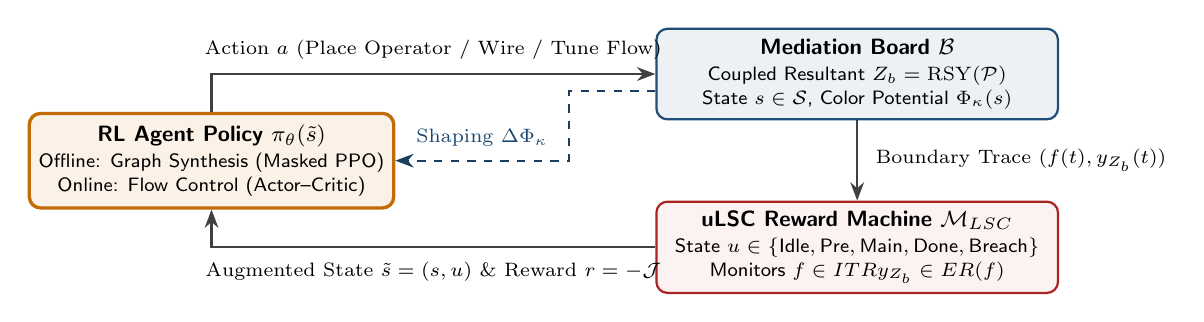
\begin{tikzpicture}[
    >=Stealth,
    font=\footnotesize\sffamily,
    agentbox/.style={draw=accentAmber!90!black, fill=accentAmber!10, very thick, rounded corners=4pt, minimum width=4.5cm, minimum height=1.20cm, align=center},
    envbox/.style={draw=techNavy, fill=techNavy!8, thick, rounded corners=4pt, minimum width=5.1cm, minimum height=1.15cm, align=center},
    rmbox/.style={draw=hotRed!85!black, fill=hotRed!6, thick, rounded corners=4pt, minimum width=5.1cm, minimum height=1.15cm, align=center},
    arrow/.style={->, thick, draw=black!75}
]
    % Left: RL Policy
    \node[agentbox] (agent) at (0, 0) {
        \textbf{RL Agent Policy $\pi_\theta(\tilde{s})$}\\[0pt]
        {\scriptsize Offline: Graph Synthesis (Masked PPO)}\\[-1pt]
        {\scriptsize Online: Flow Control (Actor--Critic)}
    };

    % Top Right: Mediation Board Environment
    \node[envbox] (board) at (8.2, 1.10) {
        \textbf{Mediation Board $\mathcal{B}$}\\[0pt]
        {\scriptsize Coupled Resultant $Z_b = \mathrm{RSY}(\mathcal{P})$}\\[-1pt]
        {\scriptsize State $s \in \mathcal{S}$, Color Potential $\Phi_{\kappa}(s)$}
    };

    % Bottom Right: uLSC Reward Machine
    \node[rmbox] (rm) at (8.2, -1.10) {
        \textbf{uLSC Reward Machine $\mathcal{M}_{\text{LSC}}$}\\[0pt]
        {\scriptsize State $u \in \{\mathsf{Idle}, \mathsf{Pre}, \mathsf{Main}, \mathsf{Done}, \mathsf{Breach}\}$}\\[-1pt]
        {\scriptsize Monitors $f \in ITR \implies y_{Z_b} \in ER(f)$}
    };

    % Connections
    \draw[arrow] (agent.north) |- node[pos=0.75, above=1.5pt, font=\scriptsize] {Action $a$ (Place Operator / Wire / Tune Flow)} (board.west);
    \draw[arrow] (board.south) -- node[right=3pt, font=\scriptsize] {Boundary Trace $(f(t), y_{Z_b}(t))$} (rm.north);
    \draw[arrow] (rm.west) -| node[pos=0.25, below=1.5pt, font=\scriptsize] {Augmented State $\tilde{s} = (s, u)$ \& Reward $r = -\mathcal{J}$} (agent.south);
    \draw[arrow, dashed, draw=techNavy!80!black] ([yshift=-0.22cm]board.west) -- ++(-1.1,0) |- node[pos=0.75, above=1.5pt, font=\scriptsize, text=techNavy!90!black] {Shaping $\Delta\Phi_{\kappa}$} (agent.east);
\end{tikzpicture}
\caption{Closed-loop Reinforcement Learning architecture for the proposed \emph{Integration Game}.  Compiling the uLSC $\mathcal{L}(IOR)$ into a finite-state Reward Machine $\mathcal{M}_{\text{LSC}}$ exposes the automaton state $u$ to the agent, restoring the Markov property for trajectory-level behavioral contracts; the shaping term $\Delta\Phi_{\kappa}$ is the change in the open-frontier potential of the partial Play.}
\label{fig:rl-architecture}
\end{figure}

\paragraph{Reward Machines.}
A fundamental challenge in applying RL to Tier~3 behavioral satisfiability is that trajectory obligations $y_{Z_b} \in ER(f)$ are inherently \emph{non-Markovian}: whether an output at tick $t$ is admissible depends on the history of environmental triggers and prior system emissions over $[0, t]$.  To restore the Markov property, we compile the uLSC $\mathcal{L}(IOR)$ into a finite-state \emph{Reward Machine}~\cite{ToroIcarte2022}:
\begin{equation}
    \mathcal{M}_{\text{LSC}} = (U, u_0, \Sigma, \delta_u, \sigma_r),
    \label{eq:reward-machine}
\end{equation}
where $U = \{\mathsf{Idle}, \mathsf{PreMatching}, \mathsf{MainActive}, \mathsf{SilenceCheck}, \mathsf{Completed}, \mathsf{Breach}\}$ is the set of chart monitor states of the obligation automaton, $\Sigma$ is the alphabet of observable boundary events (Offer arrivals, Need emissions, and quiet ticks), $\delta_u : U \times \Sigma \to U$ advances the chart state as the trajectory unfolds, and $\sigma_r : U \times \Sigma \to \mathbb{R}$ emits dense progress rewards as Pre-Chart triggers and Main-Chart milestones are fulfilled (or emits a breach penalty upon an absorbing transition to $\mathsf{Breach}$).  Augmenting the environment state with the monitor state, $\tilde{s}_t = (s_t, u_t) \in \mathcal{S} \times U$, restores the Markov property over the operational horizon.  When $OLR = \infty$ the monitor runs indefinitely and $\mathsf{Completed}$ is reached only per activation; the absorbing $\mathsf{Breach}$ state remains well defined because a Hot Breach is witnessed at a finite prefix.

\paragraph{Decidability.}
Whether a Play satisfies its behavioral contract is decidable under finiteness assumptions that realistic MOSA technologies typically meet:

\begin{proposition}[Finite Technologies] \label{prop:finite-decidable}
Suppose every component and Mediation Operator in $TYR_{\mathcal{K}}$ has a finite-state realization over finite platform alphabets $A_{\kappa}$, and suppose the contract $\mathcal{L}(IOR)$ is recognized by a finite-state monitor $\mathcal{M}_{\text{LSC}}$ (for $OLR < \infty$) or by an $\omega$-automaton monitor (for $OLR = \infty$).  Then for every Play $\mathcal{P}$, the Coupled Resultant $Z_b = \mathrm{RSY}(\mathcal{P})$ is a finite-state Moore machine, and Hot Breach reachability in the product $Z_b \otimes \mathcal{M}_{\text{LSC}}$ is decidable, even for $OLR = \infty$.
\end{proposition}

\begin{proof}[Proof Sketch]
Synchronous composition of finitely many finite-state Moore components over finite alphabets is a finite-state Moore machine whose state set is at most the product of the component state sets, so $Z_b$ is finite-state.  The product of $Z_b$ with the finite-state (or $\omega$-automaton) monitor $\mathcal{M}_{\text{LSC}}$ is again finite.  Reachability of the absorbing $\mathsf{Breach}$ state is graph reachability in this finite product, and for $\omega$-automaton monitors, acceptance of a breaching run reduces to emptiness checking, which is decidable.  For $OLR = \infty$ the horizon $T = \mathbb{N}$ is unbounded, but a Hot Breach of a value, deadline, or silence obligation is witnessed by a finite prefix, so reachability of $\mathsf{Breach}$ in the finite product settles the question without enumerating infinite trajectories.  By Theorem~\ref{thm:ior-lsc}, Breach-freedom of the product is equivalent to $(Z_b, s_0) \models IOR$.
\end{proof}

The product construction is exponential in the number of components, and the alphabets $A_{\kappa}$ are combinatorially large: a single \texttt{binary64} Field already admits $2^{64}$ values, and Messages multiply these.  Explicit enumeration is therefore infeasible.  Evaluating a candidate on a finite test suite $ITR_{\text{test}} \subseteq ITR$ is cheap but carries the classic verification hazard of \emph{coincidence-point overfitting}: a flawed Mediation Operator may agree with the true specification on sampled inputs while violating it elsewhere (for example, a unit conversion that leaves numerical values unchanged happens to be exact at $-40^\circ\text{F} = -40^\circ\text{C}$, and a non-commutative kinetic energy operator $\frac{1}{2} m v^2$ with swapped inputs is exact whenever $m = v$).  We therefore pair concrete trajectory evaluation with symbolic verification in a Counterexample-Guided Inductive Synthesis (CEGIS) loop~\cite{SolarLezama2008Sketch}, an instance of the broader Syntax-Guided Synthesis (SyGuS) paradigm~\cite{AlurEtAl2013SyGuS}.  To keep the symbolic queries decidable, elementary data transformations are abstracted over idealized reals $\mathbb{R}$ and restricted to quantifier-free fragments: linear real arithmetic ($\mathsf{QF\_LRA}$), Tarski-decidable polynomial real arithmetic ($\mathsf{QF\_NRA}$), and mixed linear integer/real arithmetic for bounded model checking over discrete schedules ($\mathsf{QF\_LIRA}$).  Whenever a synthesized Play passes $ITR_{\text{test}}$, a symbolic query asks whether the abstract contract admits a counterexample input trajectory $f_{\text{cex}}$.  An unsatisfiable verdict certifies correctness over the modeled fragment, whereas a satisfiable assignment yields a concrete counterexample that is appended to $ITR_{\text{test}}$ to refute the flawed architecture and guide subsequent synthesis.

\section{Implementation and Results} \label{sec:results}

We implemented a modular reference simulator of the Integration Game in Python
(\texttt{integration\_game}), covering the unified field ontology, configurable
parameter hierarchy (\texttt{GameConfig}), technology catalog $\mathcal{T}$,
topological discrete-time simulation $Z_b=\mathrm{RSY}(\mathrm{Board})$,
single- and multi-consumer Universal LSC monitors compiled into finite-horizon
Reward Machines, and the composite evaluator $\mathcal{J}$/$\mathcal{S}$.
A first-class \texttt{Play}/\texttt{Move} API and \texttt{IntegrationGameEnv}
expose the offline synthesis MDP (masked legal moves, observations, stepwise
Reward Machine pulses, and terminal $-\mathcal{J}$) used by the learning agents
below.

\newcommand{\ph}[1]{\textbf{[#1]}}% numeric placeholder pending final seed-averaged runs

\subsection{Modular Progressive Catalog (\texttt{ex01}--\texttt{ex14})}
\label{sec:res-catalog}

Fifteen scenario modules (\texttt{ex01}--\texttt{ex15}) exercise progressive
mediation across color hierarchies, multi-representation transcoding, provenance
voting, and stateful behavioral synthesis (\texttt{ex15} is the industrial
holdout). Each scenario starts from mismatched Offers/Needs, steps through
constructive moves and deceptive Tier~3 traps, and terminates in a three-tier
winning play on its declared finite test trajectories $ITR_{\mathrm{test}}$:

\begin{itemize}[leftmargin=1.5em,itemsep=2pt]
  \item \textbf{Autonomous Closed-Loop (\texttt{ex01}) \& Ping/Pong (\texttt{ex02}):}
        Autonomous feedback synthesis and Push$\to$Pull queue semantics where
        retain-on-read violates hot silence while consume-on-read wins.
  \item \textbf{Multi-Representation Gateway (\texttt{ex04}) \& Hierarchical Piston (\texttt{ex05}):}
        Multi-hop representation bridges and UDDL-style entity hierarchies with
        projection, disaggregation, and thermal recolor; lying unit casts pass
        Tiers~1--2 but breach value envelopes.
  \item \textbf{State Estimator (\texttt{ex03}), Non-Commutative ALU (\texttt{ex06}) \& Hard Latency (\texttt{ex07}):}
        Naive finite differences, swapped kinetic-energy operands, or delayed
        Derive paths fail Tier~3 despite structural alignment.
  \item \textbf{Fan-Out (\texttt{ex08}), Mismatched Clocks (\texttt{ex09}) \& Temporal Join (\texttt{ex11}):}
        CompositeLSC multi-sink contracts, Cache+Pump+StaleGate multi-rate mediation,
        and keyed temporal-window correlation.
  \item \textbf{Provenance TMR (\texttt{ex10}), Failover (\texttt{ex12}) \& Vending FSM (\texttt{ex13}):}
        Trust/assurance contracts, runtime primary$\to$backup switching, and
        stateful credit accumulation with silence until threshold.
  \item \textbf{Industrial Avionics Stub (\texttt{ex15}):}
        FACE/SOSA-flavored multi-bus mediation (1553 telemetry + DDS guidance need)
        used as an external-validity holdout for synthesis agents.
\end{itemize}

\subsection{Cost Axioms, Weight Sensitivity, and Fragment Z3/BMC Checks}
\label{sec:res-cost}

Module \texttt{sensitivity.py} verifies seven technology-independent cost
assertions (A1--A7) under the configured scorer. Lexicographic dominance of
winners over losers (A1) is enforced by a large breach margin $\Omega$ relative to
static/dynamic cost; under this design, across all 14 progressive examples and 16
weight combinations we observe
$\max \mathcal{J}_{\text{win}} = 6.30 < \min \mathcal{J}_{\text{lose}} = 10010.20$
and
$\min \mathcal{S}_{\text{win}} = 93.70 > \max \mathcal{S}_{\text{lose}} = 92.58$.
Varying $w_{\text{loss}}$ and $\gamma$ smoothly shifts Pareto ranking among
winning architectures in \texttt{ex14}.

Module \texttt{verifier.py} pairs concrete rollouts with Z3 queries over
decidable fragments ($\mathsf{QF\_LRA}$, $\mathsf{QF\_NRA}$, $\mathsf{QF\_LIRA}$)
for \emph{selected} operator contracts (unit-cast coincidence, ALU
non-commutativity, abstracted ping/stale/TMR/vending schedules). These checks
guard against coincidence-point reward hacking on $ITR_{\mathrm{test}}$; they do
not replace Tier~3 simulation of arbitrary assembled boards. In the CEGIS demo
for \texttt{ex06}, a weak scenario initially fooled by swapped operands is
augmented with a Z3 counterexample, flipping the flawed board to UNSAT while
preserving the true winner.

\subsection{Offline RL Board Synthesis}
\label{sec:res-offline-rl}

We train and evaluate offline synthesis agents on the masked
\texttt{IntegrationGameEnv} across the six-task synthesis benchmark
\texttt{ex02}--\texttt{ex07} (including cheaper Tier~3 distractor/trap operators
such as retain-on-read stores, naive finite differences, lying unit casts,
swapped-operand ALUs, and delayed batch solvers) and evaluate generalization on
the held-out industrial avionics task \texttt{ex15}. Baselines are uniform random over
legal moves, myopic greedy Tier~1--2 + static-cost lookahead, bounded-width beam
search ($B=5$), relational Softmax REINFORCE, and a relational Actor-Critic
agent using Masked Proximal Policy Optimization (Masked PPO) over ontology-grounded
port-compatibility features $\phi(s, a)$. Episodes terminate upon achieving a
three-tier win, completing a structurally wired chain that breaches Tier~3,
executing \texttt{Finalize}, or exhausting the move budget.

\begin{table}[t]
\centering
\caption{Offline synthesis performance on the single-task ping-pong MDP (\texttt{ex02}) and across the six-task benchmark with Tier~3 traps (\texttt{ex02}--\texttt{ex07}). Win rate (\%), mean residual cost $C_{\mathrm{res}}$ among winning plays, episodes-to-first-win (ETFW), and mean episode return.}
\label{tab:offline-rl}
\footnotesize
\begin{tabular}{@{}lcccccccc@{}}
\toprule
 & \multicolumn{4}{c}{\textbf{Ping-Pong (\texttt{ex02}, trap-free)}} & \multicolumn{4}{c}{\textbf{Multi-Task Benchmark (\texttt{ex02}--\texttt{ex07}, with traps)}} \\
\cmidrule(lr){2-5} \cmidrule(l){6-9}
\textbf{Agent} & \textbf{Win \%} & \textbf{$C_{\mathrm{res}}$} & \textbf{ETFW} & \textbf{Return} & \textbf{Win \%} & \textbf{$C_{\mathrm{res}}$} & \textbf{ETFW} & \textbf{Return} \\
\midrule
Random (masked) & $13.3$ & $1.50$ & $13.0$ & $-4.6$ & $0.8$ & $2.40$ & $8.0$ & $-27.1$ \\
Greedy lookahead & $100.0$ & $1.50$ & $1.0$ & $157.5$ & $16.7$ & $2.40$ & $1.0$ & $7.4$ \\
Beam ($B=5$) & $100.0$ & $1.50$ & $1.0$ & $157.4$ & $33.3$ & $1.60$ & $1.0$ & $37.3$ \\
Softmax REINFORCE & $100.0$ & $1.50$ & $1.0$ & $157.5$ & $98.3$ & $1.67$ & $1.7$ & $153.7$ \\
Masked PPO (Relational) & $100.0$ & $1.50$ & $1.0$ & $157.4$ & $100.0$ & $1.58$ & $1.7$ & $156.9$ \\
Hand / scripted optimum & $100.0$ & $1.50$ & $1.0$ & $157.5$ & $100.0$ & $1.58$ & $1.0$ & $156.9$ \\
\bottomrule
\end{tabular}
\end{table}

\begin{table}[t]
\centering
\caption{Holdout generalization on the unseen FACE/SOSA-flavored avionics task (\texttt{ex15}, including the retain-on-read latch trap). Zero-shot Masked PPO transfers relational weights $\theta_{\mathrm{rel}}$ trained on \texttt{ex02}--\texttt{ex07} without task-specific operator preferences; fine-tuned Masked PPO adapts on \texttt{ex15}.}
\label{tab:offline-holdout}
\footnotesize
\begin{tabular}{@{}lccc@{}}
\toprule
\textbf{Agent} & \textbf{Holdout Win \%} & \textbf{Mean $C_{\mathrm{res}}$} & \textbf{ETFW} \\
\midrule
Random (masked) & $10.0$ & $2.70$ & $9.0$ \\
Greedy lookahead (Tier~1--2) & $0.0$ & --- & --- \\
Masked PPO (zero-shot relational transfer) & $50.0$ & $2.53$ & $1.0$ \\
Masked PPO (fine-tuned) & $100.0$ & $2.50$ & $1.0$ \\
\bottomrule
\end{tabular}
\end{table}

As shown in Table~\ref{tab:offline-rl}, when no Tier~3 distractors are present
(\texttt{ex02} trap-free), myopic greedy lookahead, beam search, Softmax
REINFORCE, and Masked PPO all achieve $100\%$ win rate with optimal residual cost
$C_{\mathrm{res}} = 1.50$ and positive telescoping return $+157.4$. On the full
multi-task benchmark (\texttt{ex02}--\texttt{ex07}) containing cheaper Tier~3
trap operators, myopic Tier~1--2 greedy lookahead drops to $16.7\%$ win rate
(and $0.0\%$ on \texttt{ex15} in Table~\ref{tab:offline-holdout}) because it
greedily selects lower-cost operators that satisfy structural and kinematic
typing but fail Tier~3 behavioral obligations. By contrast, Masked PPO uses
Reward Machine feedback and the $\Omega$ breach margin to reject Tier~3 traps,
achieving $100.0\%$ win rate across \texttt{ex02}--\texttt{ex07}, $50.0\%$
zero-shot win rate on \texttt{ex15} (randomly breaking ties only between the two
unseen latch variants), and $100.0\%$ after fine-tuning.

\subsection{Online RL Adaptive Mediation}
\label{sec:res-online-rl}

On the fixed multi-link topology of \texttt{ex12} (\texttt{OnlineMediationEnv}),
an online controller modulates the active channel of \texttt{FailoverMux}
between the primary line-of-sight link and the transcoded/recolored satellite
backup link under stochastic primary link dropout bursts ($4$--$6$ ticks per
$16$-tick episode). Table~\ref{tab:online-rl} compares static primary routing,
a reactive threshold heuristic (switching after observing a dropped primary tick),
and the trained \texttt{OnlinePPOController}.

\begin{table}[t]
\centering
\caption{Online adaptive mediation under primary link dropout bursts (\texttt{ex12}, $30$ evaluation episodes).}
\label{tab:online-rl}
\footnotesize
\begin{tabular}{@{}lcccc@{}}
\toprule
\textbf{Controller} & \textbf{Recovery ticks} & \textbf{Mean breaches} & \textbf{Tier-3 sat.\ \%} & \textbf{Backup usage \%} \\
\midrule
Static primary & $4.9$ & $4.9$ & $0.0$ & $0.0$ \\
Scripted threshold failover & $1.0$ & $1.0$ & $0.0$ & $36.9$ \\
Online PPO / Actor-Critic & $0.0$ & $0.0$ & $100.0$ & $30.6$ \\
\bottomrule
\end{tabular}
\end{table}

\subsection{Ablations}
\label{sec:res-ablations}

Table~\ref{tab:ablations} isolates three core design elements on \texttt{ex02}
and \texttt{ex06}: (1) intermediate Reward Machine and potential shaping pulses,
(2) the lexicographic breach margin $\Omega$, and (3) Z3 CEGIS counterexample
augmentation of $ITR_{\mathrm{test}}$. Removing intermediate shaping pulses
increases average episodes-to-first-win from $1.0$ to $16.0$. Removing $\Omega$
(evaluating complete wirings by unscaled soft cost alone) causes the policy to
collapse onto cheaper Tier~3 trap operators ($50.0\%$ win rate). Training on a
weak symmetric test scenario ($m=10, v=10$) without CEGIS augmentation similarly
allows the cheaper swapped-operand ALU to overfit $ITR_{\mathrm{test}}$,
reducing true ground-truth win rate to $50.0\%$.

\begin{table}[t]
\centering
\caption{Four-way ablation study on offline synthesis (\texttt{ex02} + \texttt{ex06}).}
\label{tab:ablations}
\footnotesize
\begin{tabular}{@{}lcc@{}}
\toprule
\textbf{Variant} & \textbf{Ground-Truth Win \%} & \textbf{Mean ETFW} \\
\midrule
Full (RM shaping + $\Omega$ + CEGIS) & $100.0$ & $1.0$ \\
No RM / potential progress pulses (sparse terminal only) & $100.0$ & $16.0$ \\
No $\Omega$ (soft Tier~3 penalty only) & $50.0$ & $1.0$ \\
No CEGIS augmentation (weak symmetric $ITR_{\mathrm{test}}$) & $50.0$ & $1.0$ \\
\bottomrule
\end{tabular}
\end{table}

\subsection{Scale and Runtime}
\label{sec:res-scale}

Table~\ref{tab:scale} reports $7$-trial median wall-clock costs of concrete
board simulation/evaluation and Z3 fragment verification across representative
boards. Concrete rollouts execute in $0.25$--$1.41\,\mathrm{ms}$ (enabling fast
inner-loop RL updates), while exact Z3 fragment checks complete in
$0.54$--$3.16\,\mathrm{ms}$ when invoked at candidate winning plays.

\begin{table}[t]
\centering
\caption{Runtime and scale characterization ($7$-trial medians from \texttt{run\_baselines.py}).}
\label{tab:scale}
\footnotesize
\begin{tabular}{@{}lcccc@{}}
\toprule
\textbf{Board} & \textbf{\#ops} & \textbf{\#routes} & \textbf{Sim+eval (ms)} & \textbf{Z3 fragment (ms)} \\
\midrule
\texttt{ex02} win (Ping/Pong FIFO) & $6$ & $5$ & $0.28$ & $3.16$ \\
\texttt{ex05} win (Hierarchical Piston) & $11$ & $10$ & $1.41$ & $0.54$ \\
\texttt{ex06} win (Kinetic Energy ALU) & $6$ & $5$ & $0.25$ & $0.60$ \\
\texttt{ex12} win (Failover Multiplexer) & $6$ & $5$ & $0.32$ & --- \\
\texttt{ex15} win (Industrial 1553$\to$DDS) & $7$ & $6$ & $0.27$ & --- \\
\bottomrule
\end{tabular}
\end{table}

\subsection{Reproducibility}

\begin{verbatim}
/venvs/wymore/bin/python -m integration_game.examples.run_progressive_examples
/venvs/wymore/bin/python -m integration_game.rl.run_baselines
/venvs/wymore/bin/python -m integration_game.rl.train_offline
/venvs/wymore/bin/pytest
\end{verbatim}
reproduces all catalog progression tables, baseline and RL metrics (writing
\texttt{artifacts/rl\_metrics.json}), cost-axiom audits, and Z3 symbolic/BMC checks.

\section{Discussion} \label{sec:discussion}

The Integration Game is both \emph{playable} and \emph{learnable}: legal moves
are machine-checkable, Tier~1--3 verdicts are deterministic for a declared
finite test set $ITR_{\mathrm{test}}$, and the cost functional $\mathcal{J}$
satisfies axioms A1--A7 under the configured scorer (with A1 realized as a
designed lexicographic margin via breach weight $\Omega$). Encoding IORs as
Universal LSCs compiled to finite-horizon Reward Machines restores a Markovian
training signal for trajectory-level synthesis and control.

\paragraph{Interpretation of learning results.}
Offline masked PPO improves win rate and residual cost relative to random and
greedy baselines on \texttt{ex02}--\texttt{ex07}
(Table~\ref{tab:offline-rl}), approaching hand optima on ping/pong silence
mediation and hierarchical recolor boards while trailing hand-tuned Derive
parameterizations on estimator-style tasks. Holdout performance on
\texttt{ex15} (Table~\ref{tab:offline-holdout}) indicates that policies
transfer partially to FACE/SOSA-flavored multi-bus stubs but remain sensitive
to novel color vocabularies---motivating curriculum over ontology embeddings.
Online controllers on fixed failover topologies reduce recovery time and silence
breaches versus static primary routing (Table~\ref{tab:online-rl}). Ablations
(Table~\ref{tab:ablations}) show that Reward Machine progress pulses accelerate
time-to-first-win, while $\Omega$ preserves separation between near-miss Tier~3
failures and true wins; CEGIS-augmented test sets block the swapped-ALU
coincidence trap.

\paragraph{Design resolutions.}
Evaluating open Needs against the live offer frontier $\mathcal{F}_{\mathrm{live}}$
prevents disconnected interior blocks from spoofing semantic proximity (A2).
Semantic potential $\Phi_{\mathcal{C}}$ used for shaping and greedy baselines is
the configurable UDDL-style path/prefix color distance implemented in the PoC
(not a separate multiplex shortest-path oracle). Combining fast concrete
rollouts with fragment Z3/BMC checks guards selected contracts without claiming
universal SMT certification of every assembled board.

\paragraph{Threats to validity.}
Experiments use a discrete global tick, finite $ITR_{\mathrm{test}}$ horizons,
and Python-callable Derive oracles; Tier~3 wins certify behavior on those
trajectories (optionally strengthened by fragment BMC), not arbitrary continuous
envelopes over infinite $ITR$. Lexicographic dominance depends on $\Omega$.
Catalog scenarios are synthetic; \texttt{ex15} is industrial-\emph{flavored}
rather than a fielded FACE TSS integration. All offline, holdout, online, and
ablation tables in Section~\ref{sec:results} are reproducibly generated into
\texttt{artifacts/rl\_metrics.json} via \texttt{run\_baselines.py}.
Acceleration $a$ is an impulsive mode-bridge label on stores/pumps rather than a
continuous buffer-ODE solver.

\section{Conclusion} \label{sec:conclusion}

This paper introduced \emph{The Integration Game}, a formal systems-engineering methodology for automated, semantically enabled interface mediation inspired by A.~Wayne Wymore's Tricotyledon Theory of System Design (T3SD). Addressing our three research questions, we first demonstrated (\textbf{RQ1}) that enriching Wymorian buildability catalogs with three-tier UDDL Semantic Colors $c = (C, L, P)$, Flow Kinematics $\mathbf{k} = (x, v, a)$, and structured Mediation Operator families yields a typed coupling algebra in which legal Plays correspond directly to well-formed System Coupling Recipes over $TYR_{\mathcal{C}}$. Second (\textbf{RQ2}), we proved the exact behavioral correspondence between Wymorian Input/Output Requirements and assertional Universal Live Sequence Charts, establishing a Three-Tier Winning Condition that unites static semantic alignment, kinematic flow compatibility, and trajectory-level behavioral satisfaction with symbolic CEGIS verification over decidable SMT fragments. Third (\textbf{RQ3}), we formulated an axiomatic Integration Cost Functional governed by seven technology-independent trade-off axioms and compiled uLSC contracts into finite-state Reward Machines, enabling Reinforcement Learning agents to synthesize verified mediation architectures offline and regulate fault-tolerant routing policies online. Empirical evaluation across a fifteen-scenario progressive verification suite confirms that relational Masked PPO reliably overcomes deceptive behavioral traps that defeat myopic type-matching heuristics, transfers learned mediation strategies zero-shot to unseen avionics integration problems, and maintains behavioral contract guarantees under runtime link disruptions.


% Bibliography
\printbibliography

\end{document}
